\section{Simulazione degli scenari e validazione}
\label{sec:scenari}
\thispagestyle{plain}

Per verificare la robustezza dell'infrastruttura Zero Trust progettata, sono stati simulati quattordici scenari operativi, organizzati per livello di difesa (dalla crittografia di trasporto fino all'analisi comportamentale ML), ognuno mirato a testare specifiche componenti difensive e logiche del sistema. Tutti gli utenti ed operatori si interfacciano inizialmente con lo stesso portale web centralizzato, protetto da autenticazione forte e controlli contestuali (mostrato in Figura~\ref{fig:login_page}).

\begin{figure}[H]
\centering
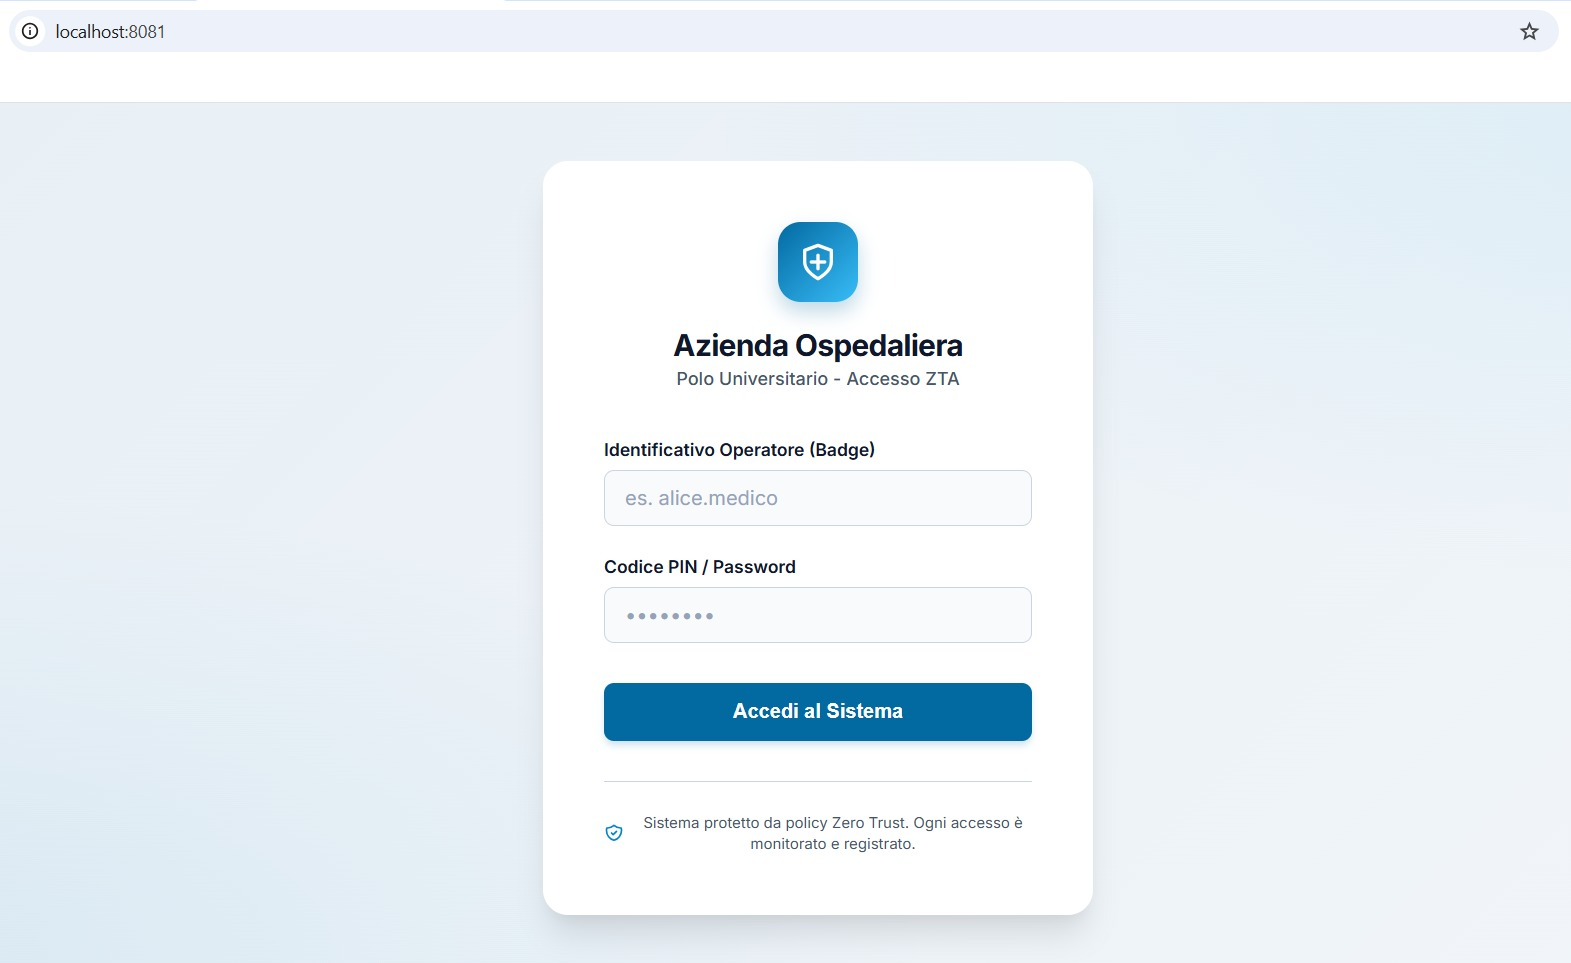
\includegraphics[width=0.85\linewidth]{capitolo4/img/login.jpeg}
\caption{Schermata del portale di login protetto.}
\label{fig:login_page}
\end{figure}

% ============================================================
% LAYER 1 — IDENTITA CRITTOGRAFICA (Envoy mTLS)
% ============================================================

\subsection{Scenario 1: Tentativo di connessione senza certificato client}
Il primo scenario ha l'obiettivo di validare il livello più esterno della difesa (Layer 1), testando la robustezza del Policy Enforcement Point (Envoy) rispetto a tentativi di connessione privi di un'identità crittografica valida. In un'architettura Zero Trust, l'assunto di base è che la rete sia intrinsecamente ostile; pertanto, il sistema deve esigere la \textit{Mutual TLS} (mTLS) prima di autorizzare o instradare qualsiasi traffico applicativo.

In questo test, viene simulata una richiesta tramite lo strumento \texttt{curl} da parte di un client che tenta di connettersi all'endpoint delle API senza fornire il proprio certificato client:

\begin{center}
\begin{minipage}{\linewidth}
\begin{ztacodebox}{curl\_no\_cert.sh}
\begin{lstlisting}[language=bash]
$ docker exec zta-client-charlie curl -k https://zta-firewall:8443/api/patients
  % Total    % Received % Xferd  Average Speed   Time    Time     Time  Current
                                 Dload  Upload   Total   Spent    Left  Speed
  0     0    0     0    0     0      0      0 --:--:-- --:--:-- --:--:--     0
curl: (56) OpenSSL SSL_read: OpenSSL/3.5.6: error:0A00045C:SSL routines::tlsv13 alert certificate required, errno 0
\end{lstlisting}
\end{ztacodebox}
\captionof{lstlisting}{Blocco preventivo a livello di trasporto per assenza di certificato client.}\label{lst:curl_no_cert}
\end{minipage}
\end{center}

Come si evince dall'output (Listato~\ref{lst:curl_no_cert}), il proxy Envoy rileva immediatamente l'assenza del certificato durante la fase di \textit{handshake} TLS. La connessione viene abortita a livello di trasporto con un alert fatale (\texttt{tlsv13 alert certificate required}), impedendo l'instaurazione del canale sicuro.

È fondamentale sottolineare l'efficienza architetturale di questo meccanismo: la richiesta HTTP (\texttt{GET /api/patients}) non viene mai elaborata. Il blocco avviene esclusivamente a livello crittografico al perimetro, garantendo che né il Policy Decision Point (OPA), né il motore di inferenza Machine Learning (Splunk), né tantomeno i servizi di backend vengano interpellati. Questo approccio \textit{fail-closed} previene attacchi di esplorazione o \textit{Denial of Service} (DoS) a livello applicativo, annullando totalmente l'\textit{overhead} computazionale per la gestione di traffico malevolo palese.

\subsection{Scenario 2: Tentativo di accesso con certificato non firmato dalla CA}
Per verificare ulteriormente il controllo sulla catena di fiducia (\textit{Trust Chain}), un secondo test simula un attaccante che tenta di presentare un certificato crittograficamente valido nella forma, ma generato autonomamente (\textit{self-signed}) e non firmato dalla \textit{Root CA} ospedaliera:

\begin{center}
\begin{minipage}{\linewidth}
\begin{ztacodebox}{curl\_fake\_cert.sh}
\begin{lstlisting}[language=bash]
$ docker exec zta-client-charlie sh -c "openssl req -x509 -newkey rsa:2048 \
  -keyout /tmp/fake.key -out /tmp/fake.crt -days 1 -nodes -subj '/CN=intruder' 2>/dev/null \
  && curl -k --cert /tmp/fake.crt --key /tmp/fake.key https://zta-firewall:8443/api/patients"
curl: (56) OpenSSL SSL_read: OpenSSL/3.5.6: error:0A000418:SSL routines::tlsv1 alert unknown ca, errno 0
\end{lstlisting}
\end{ztacodebox}
\captionof{lstlisting}{Rilevamento e blocco di un certificato estraneo alla Trust Chain ospedaliera.}\label{lst:curl_fake_cert}
\end{minipage}
\end{center}

In questo scenario, il proxy Envoy esegue una validazione rigorosa della \textit{Certificate Authority} emittente. Non riscontrando corrispondenza con la \textit{Root CA} interna configurata, il sistema interrompe immediatamente la connessione con l'errore \texttt{tlsv1 alert unknown ca}. Anche in questo caso, come nel precedente, il blocco avviene a livello di \textit{handshake} TLS, garantendo che nessuna risorsa interna (OPA o backend) venga esposta all'attaccante.

% ============================================================
% LAYER 2 — MICROSEGMENTAZIONE L3/L4 (nftables)
% ============================================================

\subsection{Scenario 3: Tentativo di bypass L4 e rilevamento attivo}
Il terzo scenario simula un tentativo di attacco in cui un utente esterno (o un dispositivo compromesso nella rete esterna, come Charlie) tenta di aggirare completamente il proxy Envoy (PEP) per connettersi direttamente al database o alle API di backend.

L'attaccante esegue una richiesta diretta tramite lo strumento \texttt{curl} dal proprio terminale verso la porta delle API:

\begin{center}
\begin{minipage}{\linewidth}
\begin{ztacodebox}{curl\_bypass.sh}
\begin{lstlisting}[language=bash]
$ docker exec -it zta-client-charlie curl -v --connect-timeout 3 http://zta-firewall:8000/api/patients
* Host zta-firewall:8000 was resolved.
*   Trying 192.168.100.4:8000...
* Connection timed out after 3002 milliseconds
* closing connection #0
curl: (28) Connection timed out after 3002 milliseconds
\end{lstlisting}
\end{ztacodebox}
\captionof{lstlisting}{Simulazione di attacco bypass diretto tramite curl dal terminale di Charlie.}\label{lst:curl_bypass}
\end{minipage}
\end{center}

Come previsto, la connessione va in timeout poiché entra in azione il firewall. \texttt{nftables} rileva la connessione diretta non autorizzata e applica la regola della trappola attiva, eseguendo il \texttt{DROP} silente dei pacchetti. Tale evento viene registrato nei log del firewall (mostrati nel Listato~\ref{lst:nftables_block_log}), evidenziando l'etichetta \texttt{[NFT-BLOCK]} e tutti i parametri del pacchetto TCP bloccato sulla porta di destinazione \texttt{8000} (DPT) proveniente dal client (\texttt{SRC=10.0.1.4}).

Si osservi che, in questo scenario di bypass di rete a livello di trasporto, lo score di rischio di Splunk non viene calcolato né registrato all'interno dei log di decisione di OPA. La connessione viene infatti intercettata e interrotta a livello di rete e trasporto (Livelli 3 e 4 del modello ISO/OSI) ad opera del firewall di rete \texttt{nftables}. Poiché i pacchetti vengono scartati (\texttt{DROP}) in kernel space prima di poter raggiungere il proxy Envoy (PEP) e attivare la catena di autorizzazione applicativa di OPA, non si innesca alcuna chiamata al proxy delle Web API ed al modello di Machine Learning. Di conseguenza, l'unica traccia dell'evento ostile in Splunk sarà limitata alle telemetrie di blocco del firewall (\texttt{[NFT-BLOCK]}) ed agli allarmi NIDS generati da Snort.

\begin{center}
\begin{minipage}{\linewidth}
\begin{ztacodebox}{nftables.log}
\begin{lstlisting}[language=bash]
Jun  2 17:03:04 f020514ab776 [NFT-BLOCK]  IN=eth2 OUT= MAC=e6:27:66:d6:b7:c9:06:c9:5e:11:ef:c1:08:00 SRC=10.0.1.4 DST=10.0.1.5 LEN=60 TOS=00 PREC=0x00 TTL=64 ID=15717 DF PROTO=TCP SPT=58384 DPT=8000 SEQ=1187313041 ACK=0 WINDOW=64240 SYN URGP=0 MARK=0
\end{lstlisting}
\end{ztacodebox}
\captionof{lstlisting}{Dettaglio del log di blocco generato da nftables per il tentativo di bypass.}\label{lst:nftables_block_log}
\end{minipage}
\end{center}

I log del firewall, insieme alle telemetrie di sistema, vengono raccolti e centralizzati in tempo reale da Fluent-Bit ed inoltrati al SIEM Splunk. La Figura~\ref{fig:splunk_logs} mostra la schermata del pannello di ricerca di Splunk Search \& Reporting, in cui si può riscontrare l'avvenuta indicizzazione dell'evento di blocco \texttt{[NFT-BLOCK]} generato dall'host \texttt{zta-firewall}.

\begin{figure}[H]
\centering
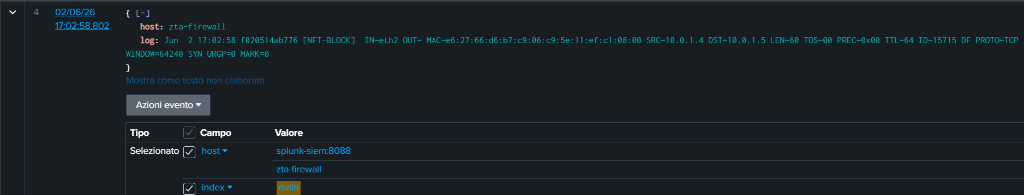
\includegraphics[width=0.95\linewidth]{capitolo4/img/splunk_logs.png}
\caption{Schermata del pannello di ricerca di Splunk che mostra il log di blocco \texttt{[NFT-BLOCK]} indicizzato.}
\label{fig:splunk_logs}
\end{figure}

Contemporaneamente, la sonda NIDS \texttt{snort} intercetta la firma del pacchetto di attacco ed esegue l'ispezione DPI, generando un allarme di intrusione. I log di alert vengono centralizzati da Fluent-Bit ed inoltrati a Splunk SIEM, il quale correla l'evento elevando il livello di rischio associato all'indirizzo IP sorgente. 

In uno scenario operativo completo, questa metrica di rischio innescherebbe un meccanismo di automazione (tramite API o webhook) verso il \textit{Policy Decision Point} (OPA), aggiornando dinamicamente la \textit{denylist} per isolare la minaccia a livello di \textit{firewall}. Pur essendo l'infrastruttura architettonicamente predisposta per tale integrazione (come illustrato nel flusso logico di Figura~\ref{fig:scenario_bypass}), l'attuale perimetro del \textit{Proof of Concept} si concentra sulla validazione della catena di rilevamento (\textit{Detection}), demandando il blocco attivo (\textit{Response} automatizzata) a sviluppi successivi.

\begin{figure}[H]
\centering
\resizebox{0.75\linewidth}{!}{%
\begin{tikzpicture}[
    % === ZONE BACKGROUNDS ===
    zonebox/.style 2 args={
        fill=#1!15!darkcharcoal, draw=#1, solid, line width=1.2pt,
        rounded corners=6pt, inner sep=12pt,
        label={[font=\footnotesize\bfseries\sffamily, text=#1]#2}
    },
    % === NODE STYLES ===
    untrustedbox/.style={draw=copper, fill=copper!8!darkcharcoal, text=cream, rounded corners=3pt,
        minimum width=2.0cm, minimum height=1.5cm, align=center, font=\scriptsize\sffamily,
        drop shadow={opacity=0.12, color=black}},
    dmzbox/.style={draw=terracotta, fill=terracotta!8!darkcharcoal, text=cream, rounded corners=3pt,
        minimum width=2.0cm, minimum height=1.5cm, align=center, font=\scriptsize\sffamily,
        drop shadow={opacity=0.12, color=black}},
    fwbox/.style={draw=copper, fill=copper!8!darkcharcoal, text=cream, rounded corners=3pt,
        minimum width=2.2cm, minimum height=1.5cm, align=center, font=\scriptsize\sffamily,
        drop shadow={opacity=0.12, color=black}},
    corebox/.style={draw=sand, fill=sand!8!darkcharcoal, text=cream, rounded corners=3pt,
        minimum width=2.2cm, minimum height=1.5cm, align=center, font=\scriptsize\sffamily,
        drop shadow={opacity=0.12, color=black}},
    controlbox/.style={draw=textmuted, fill=textmuted!8!darkcharcoal, text=cream, rounded corners=3pt,
        minimum width=2.2cm, minimum height=1.5cm, align=center, font=\scriptsize\sffamily,
        drop shadow={opacity=0.12, color=black}},
    pepbox/.style={draw=copper, fill=copper, text=white, rounded corners=4pt,
        minimum width=2.2cm, minimum height=1.5cm, align=center, font=\scriptsize\bfseries\sffamily,
        drop shadow={opacity=0.18, color=black}},
    % === ARROWS ===
    arr/.style={-{Stealth[scale=0.8]}, draw=copper, line width=1pt},
    attackarr/.style={-{Stealth[scale=0.85]}, draw=red!90!black, line width=1.5pt},
    alertarr/.style={-{Stealth[scale=0.8]}, draw=orange!90!black, line width=1.2pt},
    futurearr/.style={-{Stealth[scale=0.8]}, draw=textmuted, densely dotted, line width=1.2pt}, % STILE PER IMPLEMENTAZIONE FUTURA
    darr/.style={-{Stealth[scale=0.7]}, draw=textmuted, densely dashed, line width=0.7pt},
    lbl/.style={font=\tiny\bfseries\sffamily}
]

    % ==================== DATA PLANE (Y = 0) ====================
    \node[untrustedbox, draw=red!80!black, line width=2pt] (charlie) at (2, 2.2)
        {
\includegraphics[height=0.55cm]{capitolo2/img/charlie.png}\\[0.05cm]\textbf{Charlie}};

    \node[dmzbox, draw=textmuted, text=textmuted] (alice) at (2, 0)
        {
\includegraphics[height=0.55cm]{capitolo2/img/alice.png}\\[0.05cm]\textbf{Alice}};
    \node[dmzbox, draw=textmuted, text=textmuted] (bob)   at (2,-2)
        {
\includegraphics[height=0.55cm]{capitolo2/img/bob.png}\\[0.05cm]\textbf{Bob}};
    \node[fwbox, draw=red!80!black, line width=1.5pt]   (fw)    at (6, 0)
        {
\includegraphics[width=0.7cm]{capitolo2/img/nftables.png}\\[0.03cm]\textbf{Firewall}};

    \node[pepbox, draw=textmuted, text=textmuted] (pep) at (10, 0)
        {
\includegraphics[width=0.7cm]{capitolo2/img/envoy.png}\\[0.03cm]Envoy};

    \node[corebox, draw=textmuted, text=textmuted] (webapi)  at (14, 1.2)
        {
\includegraphics[width=0.7cm]{capitolo2/img/python.png}\\[0.03cm]\textbf{Web API}};
    \node[corebox, draw=red!80!black, line width=1.5pt] (mongodb) at (14,-1.2)
        {
\includegraphics[width=0.7cm]{capitolo2/img/mongodb.png}\\[0.03cm]\textbf{MongoDB}};

    % ==================== CONTROL PLANE ====================
    \node[controlbox, draw=orange!90!black, line width=1.5pt] (snort) at (3.5, -5)
        {
\includegraphics[width=0.7cm]{capitolo2/img/snort.png}\\[0.03cm]\textbf{Snort}};
    \node[controlbox, draw=red!80!black, line width=1.5pt] (splunk) at (3.5, -7.5)
        {
\includegraphics[width=0.7cm]{capitolo2/img/splunk.png}\\[0.03cm]\textbf{Splunk}};
    \node[controlbox, draw=orange!90!black, line width=1.2pt] (fluentbit) at (8, -7.5)
        {
\includegraphics[width=0.7cm]{capitolo2/img/fluentbit.png}\\[0.03cm]\textbf{Fluent-Bit}};
    \node[controlbox, draw=textmuted, line width=1pt] (opa) at (12.5, -7.5) % RESO NEUTRO PER INDICARE PREDISPOSIZIONE
        {
\includegraphics[width=0.7cm]{capitolo2/img/opa.png}\\[0.03cm]\textbf{OPA}};

    % ==================== ETICHETTE ====================
    \node[below=0.02cm of fw, font=\scriptsize\bfseries\sffamily\color{red!80!black}] {DROP};
    \node[below=0.02cm of snort, font=\scriptsize\bfseries\sffamily\color{orange!80!black}] {Alert Scansione};
    \node[below=0.02cm of splunk, font=\scriptsize\bfseries\sffamily\color{red!80!black}] {Rischio Max};
    \node[below=0.02cm of opa, font=\scriptsize\bfseries\sffamily\color{textmuted}] {(Predisposto)}; % MODIFICATA LABEL
    \node[below=0.02cm of mongodb, font=\scriptsize\bfseries\sffamily\color{red!80!black}] {Bloccato};

    % ==================== ZONE BACKGROUNDS ====================
    \begin{scope}[on background layer]
        \node[zonebox={copper}{above:Rete Esterna}, inner sep=7pt]          [fit=(charlie)] {};
        \node[zonebox={terracotta}{below:Rete Interna}, inner sep=7pt]  [fit=(alice)(bob)] {};
        \node[zonebox={sand}{above:Risorse Protette}]           [fit=(webapi)(mongodb)] {};
        \node[zonebox={textmuted}{below:Piano di Controllo}]    [fit=(opa)(fluentbit)(splunk)] {};
    \end{scope}

    % ==================== FLUSSI ====================
    \draw[attackarr] (charlie.east) -- node[above, lbl, pos=0.5, color=red!90!black]{TCP 8000 (Bypass)} (fw.west);
    \draw[darr] (webapi.south) -- (mongodb.north);

    \draw[attackarr] (fw.south) -- ++(0,-2.5) -| node[pos=0.2, above, lbl, color=red!80!black]{Ispezione DPI} (snort.north);
    \draw[alertarr] (snort.east) to [bend left=15] node[above, lbl, color=orange!80!black]{Alert snort.alerts} (fluentbit.north);
    \draw[alertarr] (fluentbit.west) -- node[above, lbl, color=red!70!black]{HEC Critico} (splunk.east);
    
    % FRECCIA MODIFICATA PER INDICARE SVILUPPO FUTURO
    \draw[futurearr] (splunk.south) -- ++(0,-0.8) -| node[pos=0.5, below, lbl, color=textmuted]{(Future Work) Aggiorna Denylist} (opa.south);

\end{tikzpicture}%
}
\caption{Mappatura logica dei flussi nello Scenario 3 (Tentativo di bypass e predisposizione architetturale per l'isolamento automatico).}
\label{fig:scenario_bypass}
\end{figure}

% ============================================================
% LAYER 4-7 — POLICY ZERO TRUST (Envoy + OPA + Splunk ML)
% ============================================================

\subsection{Scenario 4: Accesso legittimo da rete interna: Alice}
Il quarto scenario analizza il comportamento del sistema di fronte all'accesso di un utente autorizzato dotato di dispositivo aziendale integro, simulato dall'utente Alice.

Alice effettua la connessione dall'interno della rete aziendale presentando un certificato client contenente l'estensione crittografica del chip TPM. All'arrivo della richiesta, \texttt{envoy} estrae il certificato e calcola il fingerprinting \textit{JA3} del browser, trasmettendo i dati ad OPA. OPA contatta la Web API di \texttt{splunk} che calcola un punteggio di rischio minimo, pari a circa uno, data la totale assenza di anomalie comportamentali. Poiché il rischio è ampiamente inferiore alla soglia massima di tolleranza di cinquanta prevista per i dispositivi sicuri interni, OPA risponde con un responso positivo di \textbf{ALLOW} ed \texttt{envoy} instrada in pochissimi millisecondi la query verso il database, restituendo ad Alice i risultati richiesti con successo (mostrati in Figura~\ref{fig:alice_dashboard}). Il relativo log di OPA, indicizzato in Splunk, conferma l'esito positivo dell'operazione, la postura integra del dispositivo e il rischio complessivo calcolato (Figura~\ref{fig:splunk_alice_allowed}).

\begin{figure}[H]
\centering
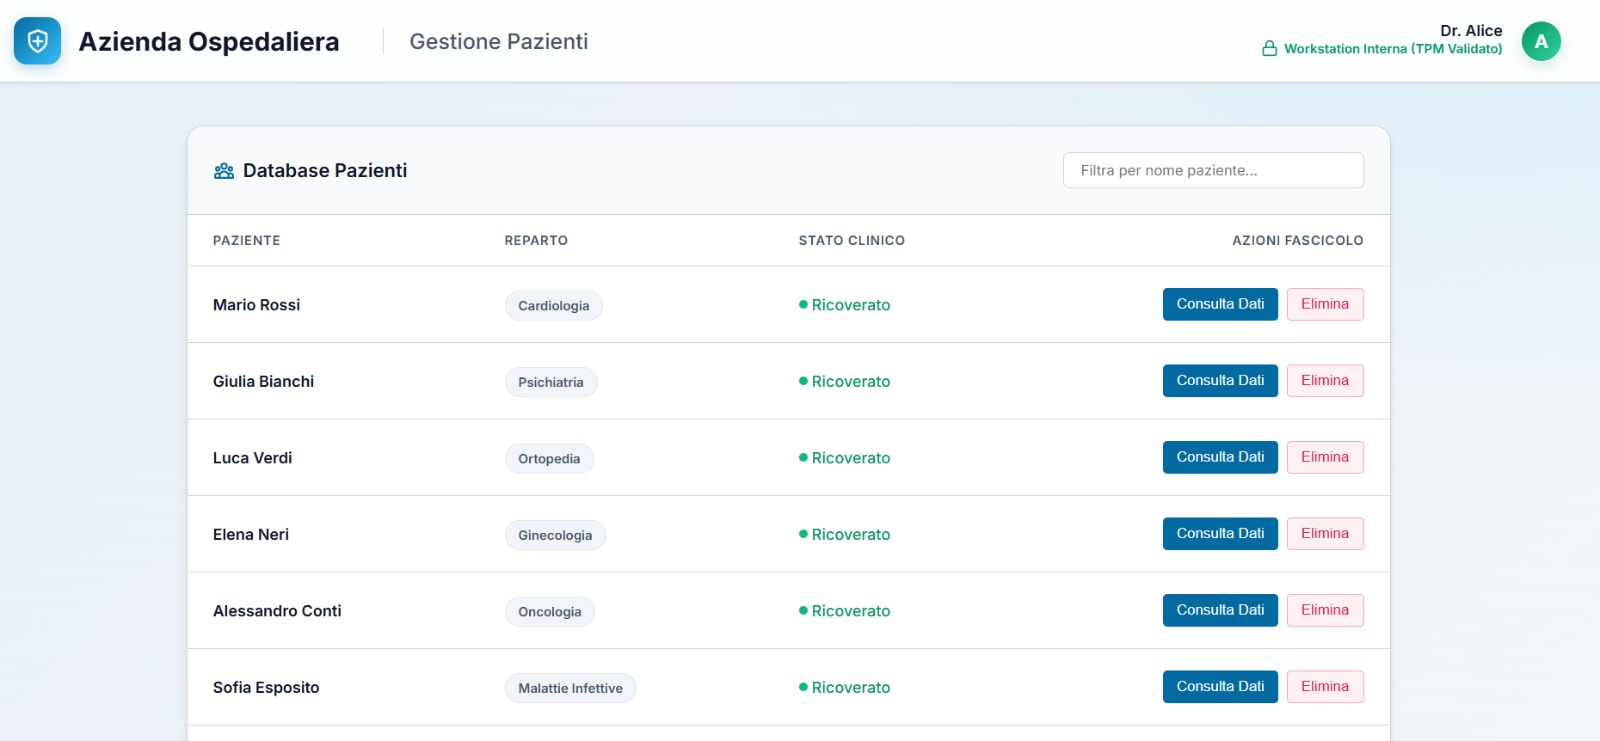
\includegraphics[width=0.85\linewidth]{capitolo4/img/alice_dashboard.png}
\caption{Interfaccia del database pazienti visualizzata con successo da Alice dopo validazione TPM e rischio minimo.}
\label{fig:alice_dashboard}
\end{figure}

\begin{figure}[H]
\centering
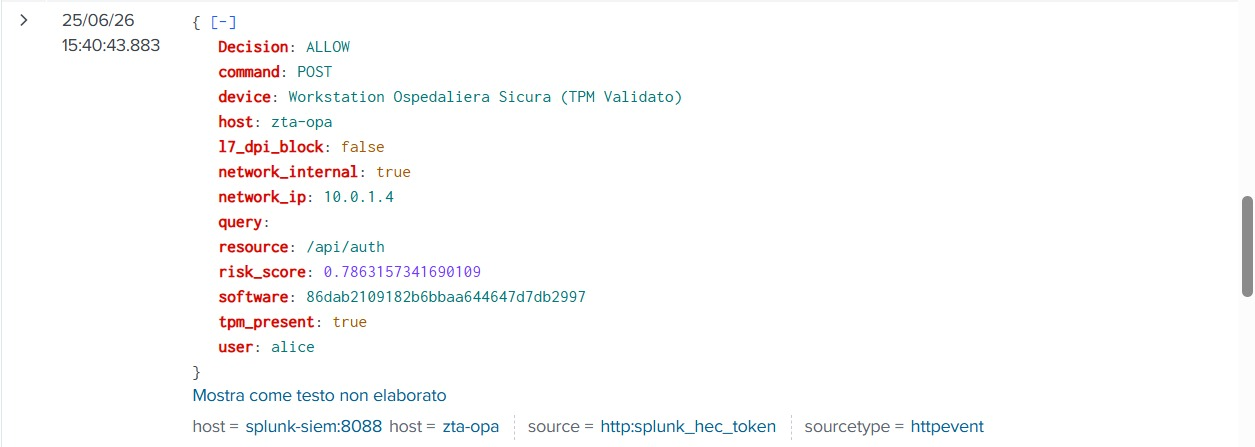
\includegraphics[width=0.9\linewidth]{capitolo4/img/splunk_alice_allowed.jpeg}
\caption{Log di autorizzazione (ALLOW) per l'accesso di Alice indicizzato in Splunk, comprensivo del risk score comportamentale calcolato ($\approx 9.96$).}
\label{fig:splunk_alice_allowed}
\end{figure}

\begin{figure}[H]
\centering
\resizebox{0.75\linewidth}{!}{%
\begin{tikzpicture}[
    zonebox/.style 2 args={
        fill=#1!15!darkcharcoal, draw=#1, solid, line width=1.2pt,
        rounded corners=6pt, inner sep=12pt,
        label={[font=\footnotesize\bfseries\sffamily, text=#1]#2}
    },
    untrustedbox/.style={draw=copper, fill=copper!8!darkcharcoal, text=cream, rounded corners=3pt,
        minimum width=2.0cm, minimum height=1.5cm, align=center, font=\scriptsize\sffamily,
        drop shadow={opacity=0.12, color=black}},
    dmzbox/.style={draw=terracotta, fill=terracotta!8!darkcharcoal, text=cream, rounded corners=3pt,
        minimum width=2.0cm, minimum height=1.5cm, align=center, font=\scriptsize\sffamily,
        drop shadow={opacity=0.12, color=black}},
    fwbox/.style={draw=copper, fill=copper!8!darkcharcoal, text=cream, rounded corners=3pt,
        minimum width=2.2cm, minimum height=1.5cm, align=center, font=\scriptsize\sffamily,
        drop shadow={opacity=0.12, color=black}},
    corebox/.style={draw=sand, fill=sand!8!darkcharcoal, text=cream, rounded corners=3pt,
        minimum width=2.2cm, minimum height=1.5cm, align=center, font=\scriptsize\sffamily,
        drop shadow={opacity=0.12, color=black}},
    controlbox/.style={draw=textmuted, fill=textmuted!8!darkcharcoal, text=cream, rounded corners=3pt,
        minimum width=2.2cm, minimum height=1.5cm, align=center, font=\scriptsize\sffamily,
        drop shadow={opacity=0.12, color=black}},
    pepbox/.style={draw=copper, fill=copper, text=white, rounded corners=4pt,
        minimum width=2.2cm, minimum height=1.5cm, align=center, font=\scriptsize\bfseries\sffamily,
        drop shadow={opacity=0.18, color=black}},
    arr/.style={-{Stealth[scale=0.8]}, draw=copper, line width=1pt},
    successarr/.style={-{Stealth[scale=0.85]}, draw=green!70!black, line width=1.5pt},
    darr/.style={-{Stealth[scale=0.7]}, draw=textmuted, densely dashed, line width=0.7pt},
    lbl/.style={font=\tiny\bfseries\sffamily}
]

    \node[untrustedbox, draw=textmuted, text=textmuted] (charlie) at (2, 2.2)
        {
\includegraphics[height=0.55cm]{capitolo2/img/charlie.png}\\[0.05cm]\textbf{Charlie}};
    \node[dmzbox, draw=green!80!black, line width=2pt] (alice) at (2, 0)
        {
\includegraphics[height=0.55cm]{capitolo2/img/alice.png}\\[0.05cm]\textbf{Alice}};
    \node[dmzbox, draw=textmuted, text=textmuted] (bob)   at (2,-2)
        {
\includegraphics[height=0.55cm]{capitolo2/img/bob.png}\\[0.05cm]\textbf{Bob}};
    \node[fwbox, draw=green!80!black, line width=1.5pt]   (fw)    at (6, 0)
        {
\includegraphics[width=0.7cm]{capitolo2/img/nftables.png}\\[0.03cm]\textbf{Firewall}};
    \node[pepbox, draw=green!80!black, line width=2pt] (pep) at (10, 0)
        {
\includegraphics[width=0.7cm]{capitolo2/img/envoy.png}\\[0.03cm]Envoy};
    \node[corebox, draw=green!80!black, line width=1.5pt] (webapi)  at (14, 1.2)
        {
\includegraphics[width=0.7cm]{capitolo2/img/python.png}\\[0.03cm]\textbf{Web API}};
    \node[corebox, draw=green!80!black, line width=1.5pt] (mongodb) at (14,-1.2)
        {
\includegraphics[width=0.7cm]{capitolo2/img/mongodb.png}\\[0.03cm]\textbf{MongoDB}};
    \node[controlbox] (snort) at (3.5, -5)
        {
\includegraphics[width=0.7cm]{capitolo2/img/snort.png}\\[0.03cm]\textbf{Snort}};
    \node[controlbox, draw=green!80!black, line width=1.5pt] (splunk) at (3.5, -7.5)
        {
\includegraphics[width=0.7cm]{capitolo2/img/splunk.png}\\[0.03cm]\textbf{Splunk}};
    \node[controlbox] (fluentbit) at (8, -7.5)
        {
\includegraphics[width=0.7cm]{capitolo2/img/fluentbit.png}\\[0.03cm]\textbf{Fluent-Bit}};
    \node[controlbox, draw=green!80!black, line width=1.5pt] (opa) at (12.5, -7.5)
        {
\includegraphics[width=0.7cm]{capitolo2/img/opa.png}\\[0.03cm]\textbf{OPA}};

    \node[below=0.02cm of alice, font=\scriptsize\bfseries\sffamily\color{green!80!black}] {TPM Validato};
    \node[below=0.02cm of pep, font=\scriptsize\bfseries\sffamily\color{green!80!black}] {VERDETTO: ALLOW};
    \node[below=0.02cm of mongodb, font=\scriptsize\bfseries\sffamily\color{green!80!black}] {Query OK};
    \node[below=0.02cm of splunk, font=\scriptsize\bfseries\sffamily\color{green!80!black}] {Rischio $\approx 1$};
    \node[below=0.02cm of opa, font=\scriptsize\bfseries\sffamily\color{green!80!black}] {Soglia $\le 50$};

    \begin{scope}[on background layer]
        \node[zonebox={copper}{above:Rete Esterna}, inner sep=7pt]          [fit=(charlie)] {};
        \node[zonebox={terracotta}{below:Rete Interna}, inner sep=7pt]  [fit=(alice)(bob)] {};
        \node[zonebox={sand}{above:Risorse Protette}]           [fit=(webapi)(mongodb)] {};
        \node[zonebox={textmuted}{below:Piano di Controllo}]    [fit=(opa)(fluentbit)(splunk)] {};
    \end{scope}

    \draw[successarr] (alice.east)   -- node[above, lbl, pos=0.5, color=terracotta]{mTLS+TPM} (fw.west);
    \draw[successarr] (fw.east) -- node[above, lbl, color=copper]{DNAT} (pep.west);
    \draw[successarr] (pep.east) -- node[above, lbl, pos=0.5, color=sand]{HTTP} (webapi.west);
    \draw[successarr] (webapi.south) -- node[right, lbl, color=sand]{TCP} (mongodb.north);
    \draw[successarr] (pep.south) -- ++(0,-2.5) -| node[pos=0.2, above, lbl, color=green!80!black]{Verifica gRPC} (opa.north);
    \draw[successarr] (opa.south) -- ++(0,-1.4) -| (splunk.south);
    \draw[darr] (fw.south)      to [bend right=15] node[right, lbl, pos=0.7, color=textmuted]{Log} (fluentbit.north);
    \draw[darr] (pep.south)     to [bend left=10]  node[right, lbl, pos=0.6, color=textmuted]{Log} (fluentbit.north);
    \draw[darr] (mongodb.south) to [bend left=15]  node[left, lbl, pos=0.4, color=textmuted]{Log}  (fluentbit.north);
    \draw[darr] (fluentbit.west) -- node[above, lbl, color=textmuted]{Inoltro Log} (splunk.east);

\end{tikzpicture}%
}
\caption{Mappatura logica dei flussi nello Scenario 4 (Accesso legittimo di Alice).}
\label{fig:scenario_alice}
\end{figure}

\subsection{Scenario 5: Blocco al login per mancanza di TPM: Bob}
Il quinto scenario testa la reazione della politica di sicurezza di fronte a un tentativo di accesso condotto tramite un dispositivo privo di chip TPM hardware, simulato dall'utente Bob.

Bob tenta di effettuare l'autenticazione utilizzando un computer personale. Sebbene il dispositivo possieda una connettività valida, il certificato presentato è privo dell'estensione di attestazione hardware TPM. All'arrivo della richiesta di login (\texttt{/api/auth}), Envoy inoltra i metadati del certificato ad OPA. Il PDP rileva la mancanza della firma hardware (\texttt{tpm\_present: false}) e, in conformità alle regole di sicurezza, definisce la variabile \texttt{is\_auth\_blocked} come \texttt{true}. Di conseguenza, la richiesta di Bob viene rigettata con un responso di \textbf{DENY} immediato al login, impedendogli l'accesso alla sessione, come illustrato nella Figura~\ref{fig:bob_blocked}.

Il log di blocco registrato in Splunk (Figura~\ref{fig:splunk_bob_blocked}) evidenzia la solidità dell'approccio Zero Trust: nonostante il profilo dell'utente non presenti anomalie storiche, il sistema assegna un \textit{Risk Score} di \texttt{100} in presenza di violazioni hardware. Questo comportamento riflette l'applicazione del principio di \textit{Short-Circuiting}: OPA rileva il vincolo hardware non soddisfatto e blocca l'accesso immediatamente, evitando chiamate ridondanti al motore di inferenza ML e garantendo che la postura del dispositivo costituisca un vincolo forte e non compensabile da altri fattori contestuali.

Dal punto di vista dell'architettura ISO/OSI, la negoziazione del canale crittografico (Livelli 5 e 6 - TLS/mTLS) tra il client e il proxy Envoy si completa con successo, poiché Bob possiede chiavi valide firmate dalla CA interna. Il diniego effettivo viene applicato esclusivamente al Livello 7 (Applicazione): il proxy Envoy, in qualità di Policy Enforcement Point (PEP), analizza la richiesta HTTP, decodifica il certificato X.509 e inoltra i metadati ad OPA (PDP). È quest'ultimo che, valutando le asserzioni di policy, impone il rifiuto logico. Il firewall di rete \texttt{nftables} non interviene in questa fase poiché l'IP di Bob rientra nei flussi di transito consentiti sulla rete interna; la protezione è dunque interamente demandata al controllo rigoroso dell'identità del dispositivo a livello applicativo.

\begin{figure}[H]
    \centering
    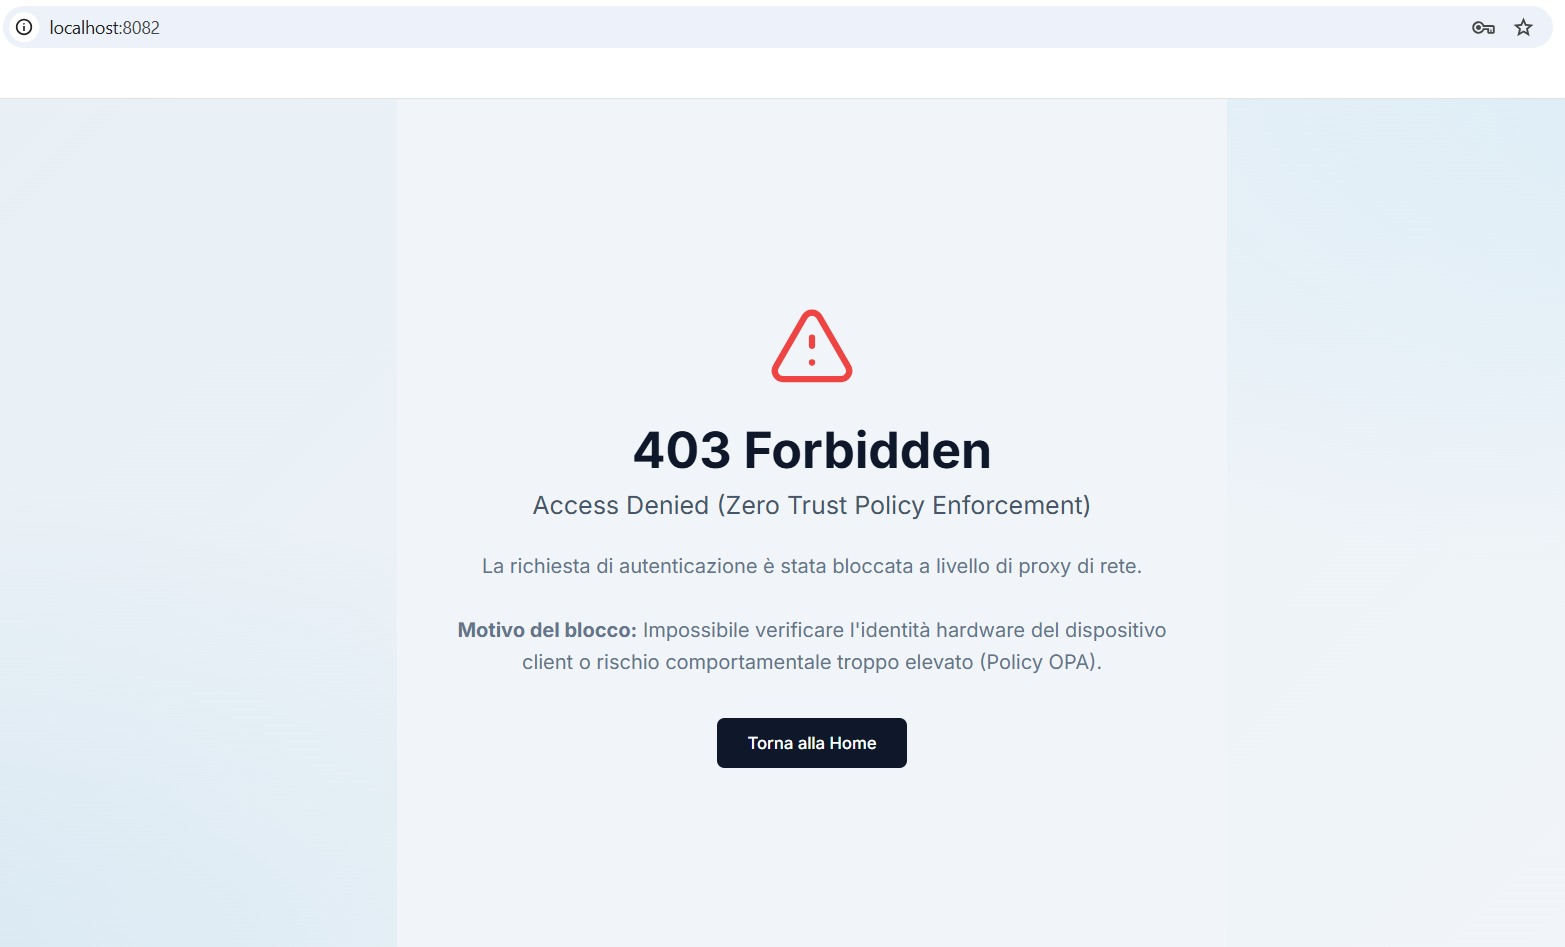
\includegraphics[width=0.85\linewidth]{capitolo4/img/bob_blocked.jpeg}
    \caption{Schermata di errore 403 Forbidden mostrata a Bob per mancata attestazione hardware del chip TPM.}
    \label{fig:bob_blocked}
\end{figure}

\begin{figure}[H]
    \centering
    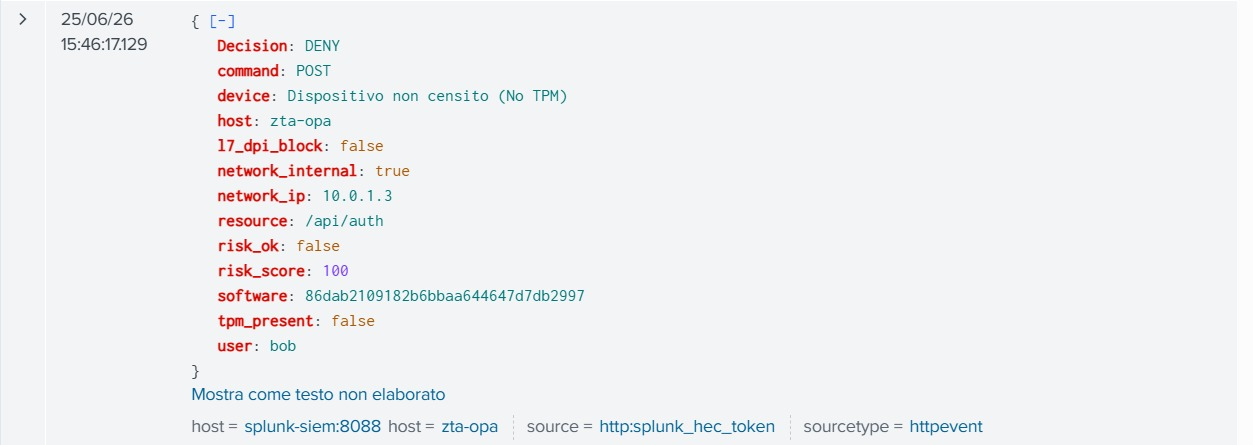
\includegraphics[width=0.9\linewidth]{capitolo4/img/splunk_bob_blocked.jpeg}
    \caption{Log di diniego (DENY) per l'accesso di Bob indicizzato in Splunk, evidenziante l'assenza della firma hardware TPM (\texttt{tpm\_present: false}) e l'assegnazione automatica del rischio massimo.}
    \label{fig:splunk_bob_blocked}
\end{figure}

\begin{figure}[H]
\centering
\resizebox{0.75\linewidth}{!}{%
\begin{tikzpicture}[
    zonebox/.style 2 args={
        fill=#1!15!darkcharcoal, draw=#1, solid, line width=1.2pt,
        rounded corners=6pt, inner sep=12pt,
        label={[font=\footnotesize\bfseries\sffamily, text=#1]#2}
    },
    untrustedbox/.style={draw=copper, fill=copper!8!darkcharcoal, text=cream, rounded corners=3pt,
        minimum width=2.0cm, minimum height=1.5cm, align=center, font=\scriptsize\sffamily,
        drop shadow={opacity=0.12, color=black}},
    dmzbox/.style={draw=terracotta, fill=terracotta!8!darkcharcoal, text=cream, rounded corners=3pt,
        minimum width=2.0cm, minimum height=1.5cm, align=center, font=\scriptsize\sffamily,
        drop shadow={opacity=0.12, color=black}},
    fwbox/.style={draw=copper, fill=copper!8!darkcharcoal, text=cream, rounded corners=3pt,
        minimum width=2.2cm, minimum height=1.5cm, align=center, font=\scriptsize\sffamily,
        drop shadow={opacity=0.12, color=black}},
    corebox/.style={draw=sand, fill=sand!8!darkcharcoal, text=cream, rounded corners=3pt,
        minimum width=2.2cm, minimum height=1.5cm, align=center, font=\scriptsize\sffamily,
        drop shadow={opacity=0.12, color=black}},
    controlbox/.style={draw=textmuted, fill=textmuted!8!darkcharcoal, text=cream, rounded corners=3pt,
        minimum width=2.2cm, minimum height=1.5cm, align=center, font=\scriptsize\sffamily,
        drop shadow={opacity=0.12, color=black}},
    pepbox/.style={draw=copper, fill=copper, text=white, rounded corners=4pt,
        minimum width=2.2cm, minimum height=1.5cm, align=center, font=\scriptsize\bfseries\sffamily,
        drop shadow={opacity=0.18, color=black}},
    arr/.style={-{Stealth[scale=0.8]}, draw=copper, line width=1pt},
    failarr/.style={-{Stealth[scale=0.85]}, draw=red!70!black, line width=1.5pt},
    blockarr/.style={-{Stealth[scale=0.7]}, draw=red!60!black, line width=1.5pt, dashed},
    darr/.style={-{Stealth[scale=0.7]}, draw=textmuted, densely dashed, line width=0.7pt},
    lbl/.style={font=\tiny\bfseries\sffamily}
]

    \node[untrustedbox, draw=textmuted, text=textmuted] (charlie) at (2, 2.2)
        {
\includegraphics[height=0.55cm]{capitolo2/img/charlie.png}\\[0.05cm]\textbf{Charlie}};
    \node[dmzbox, draw=textmuted, text=textmuted] (alice) at (2, 0)
        {
\includegraphics[height=0.55cm]{capitolo2/img/alice.png}\\[0.05cm]\textbf{Alice}};
    \node[dmzbox, draw=red!80!black, line width=2pt] (bob)   at (2,-2)
        {
\includegraphics[height=0.55cm]{capitolo2/img/bob.png}\\[0.05cm]\textbf{Bob}};
    \node[fwbox, draw=red!80!black, line width=1.5pt]   (fw)    at (6, 0)
        {
\includegraphics[width=0.7cm]{capitolo2/img/nftables.png}\\[0.03cm]\textbf{Firewall}};
    \node[pepbox, draw=red!80!black, line width=2pt] (pep) at (10, 0)
        {
\includegraphics[width=0.7cm]{capitolo2/img/envoy.png}\\[0.03cm]Envoy};
    \node[corebox, draw=textmuted, text=textmuted] (webapi)  at (14, 1.2)
        {
\includegraphics[width=0.7cm]{capitolo2/img/python.png}\\[0.03cm]\textbf{Web API}};
    \node[corebox, draw=textmuted, text=textmuted] (mongodb) at (14,-1.2)
        {
\includegraphics[width=0.7cm]{capitolo2/img/mongodb.png}\\[0.03cm]\textbf{MongoDB}};
    \node[controlbox] (snort) at (3.5, -5)
        {
\includegraphics[width=0.7cm]{capitolo2/img/snort.png}\\[0.03cm]\textbf{Snort}};
    \node[controlbox, draw=red!80!black, line width=1.5pt] (splunk) at (3.5, -7.5)
        {
\includegraphics[width=0.7cm]{capitolo2/img/splunk.png}\\[0.03cm]\textbf{Splunk}};
    \node[controlbox] (fluentbit) at (8, -7.5)
        {
\includegraphics[width=0.7cm]{capitolo2/img/fluentbit.png}\\[0.03cm]\textbf{Fluent-Bit}};
    \node[controlbox, draw=red!80!black, line width=1.5pt] (opa) at (12.5, -7.5)
        {
\includegraphics[width=0.7cm]{capitolo2/img/opa.png}\\[0.03cm]\textbf{OPA}};

    \node[below=0.02cm of pep, font=\scriptsize\bfseries\sffamily\color{red!80!black}] {VERDETTO: DENY};
    \node[below=0.02cm of mongodb, font=\scriptsize\bfseries\sffamily\color{red!80!black}] {Non Raggiunto};
    \node[below=0.02cm of splunk, font=\scriptsize\bfseries\sffamily\color{red!80!black}] {Log Ricevuto};
    \node[below=0.02cm of opa, font=\scriptsize\bfseries\sffamily\color{red!80!black}] {is\_auth\_blocked = true};

    \begin{scope}[on background layer]
        \node[zonebox={copper}{above:Rete Esterna}, inner sep=7pt]          [fit=(charlie)] {};
        \node[zonebox={terracotta}{below:Rete Interna}, inner sep=7pt]  [fit=(alice)(bob)] {};
        \node[zonebox={sand}{above:Risorse Protette}]           [fit=(webapi)(mongodb)] {};
        \node[zonebox={textmuted}{below:Piano di Controllo}]    [fit=(opa)(fluentbit)(splunk)] {};
    \end{scope}

    \draw[failarr] (bob.east)   -- node[below, lbl, pos=0.5, color=terracotta]{mTLS (No TPM)} (fw.west);
    \draw[failarr] (fw.east) -- node[above, lbl, color=copper]{DNAT} (pep.west);
    \draw[blockarr] (pep.east) -- node[above, lbl, pos=0.5, color=red!80!black]{\textbf{BLOCCATO}} (webapi.west);
    \draw[darr] (webapi.south) -- (mongodb.north);
    \draw[failarr] (pep.south) -- ++(0,-2.5) -| node[pos=0.2, above, lbl, color=red!70!black]{Verifica gRPC} (opa.north);
    \draw[darr, draw=red!70!black] (opa.south) -- ++(0,-1.4) -| node[pos=0.5, above, lbl, color=red!70!black]{Log di Blocco} (splunk.south);
    \draw[darr, draw=red!70!black] (pep.south)     to [bend left=10]  node[right, lbl, pos=0.6, color=red!70!black]{Log} (fluentbit.north);
    \draw[darr, draw=red!70!black] (fluentbit.west) -- node[above, lbl, color=red!70!black]{Inoltro Log} (splunk.east);

\end{tikzpicture}%
}
\caption{Mappatura logica dei flussi nello Scenario 5 (Blocco al login di Bob per mancanza di TPM).}
\label{fig:scenario_bob}
\end{figure}

\subsection{Scenario 6: Accesso legittimo da rete esterna: Charlie}
Il sesto scenario analizza la gestione dell'accesso remoto (Smart Working). Charlie è un operatore legittimo dell'ospedale, dotato di credenziali valide e di un dispositivo autorizzato provvisto di chip TPM. In questo caso, il sistema Zero Trust non applica un blocco preventivo al login, ma abilita un controllo adattivo basato sul rischio.

Quando Charlie si autentica da casa (rete esterna, \texttt{network\_internal: false}), il PEP (Envoy) interroga OPA fornendo il contesto di rete. Poiché il dispositivo di Charlie presenta un'attestazione hardware valida e il suo \textit{Risk Score} calcolato dal motore ML è pari a $17.7$ (valore inferiore alla soglia ristretta di $26$ prevista per gli utenti remoti), il sistema concede l'accesso al portale, come illustrato in Figura~\ref{fig:charlie_dashboard}. Il log di Splunk in Figura~\ref{fig:splunk_charlie_allowed} conferma il verdetto di \textbf{ALLOW}: il sistema riconosce che l'utente è remoto, ma la validità della postura (TPM presente) e il basso punteggio di rischio comportamentale permettono di derogare al blocco totale, garantendo la continuità operativa in sicurezza.

\begin{figure}[H]
    \centering
    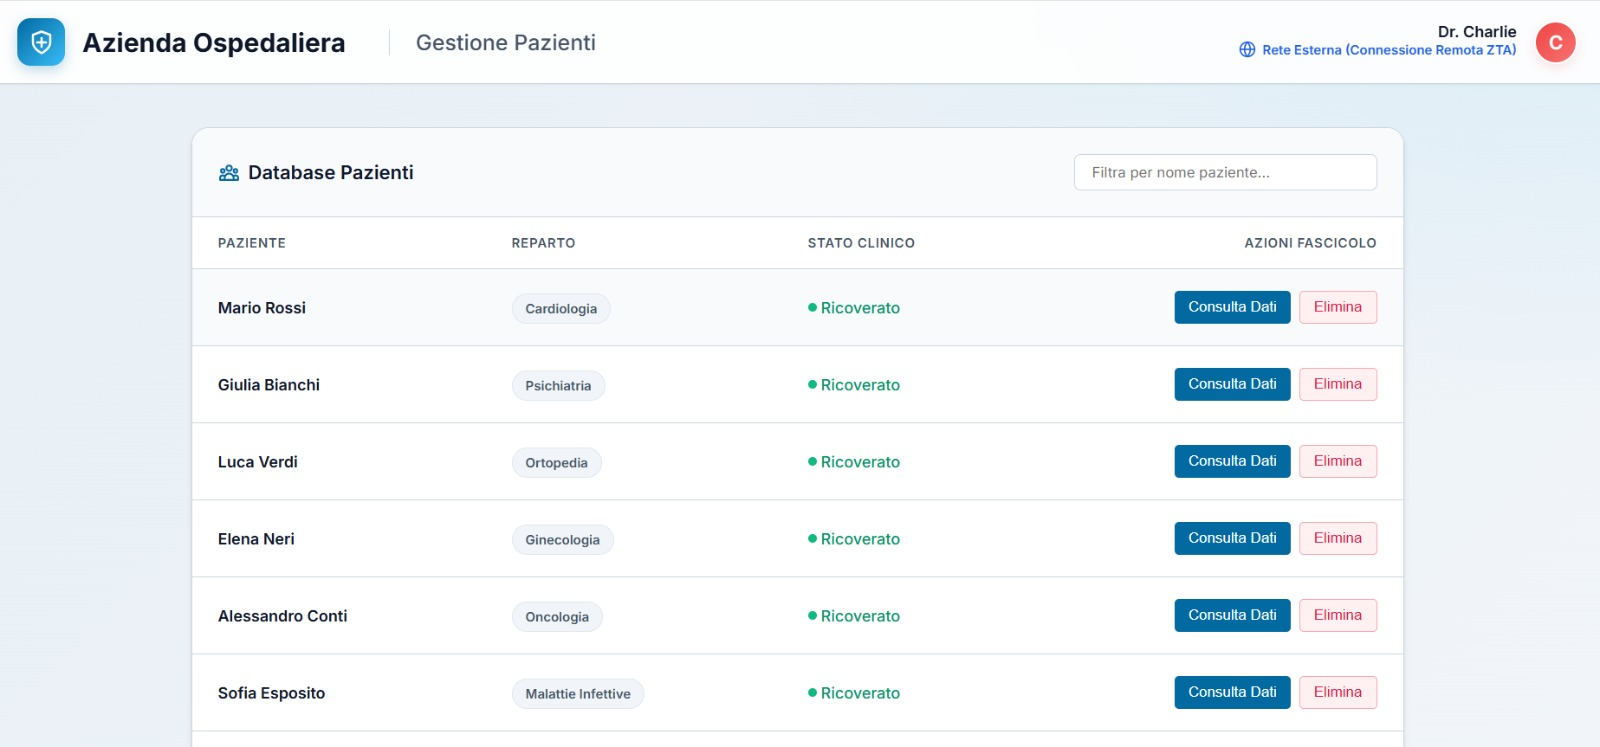
\includegraphics[width=0.85\linewidth]{capitolo4/img/charlie_dashboard.jpeg}
    \caption{Dashboard di Charlie dopo l'autenticazione riuscita da rete esterna.}
    \label{fig:charlie_dashboard}
\end{figure}

\begin{figure}[H]
    \centering
    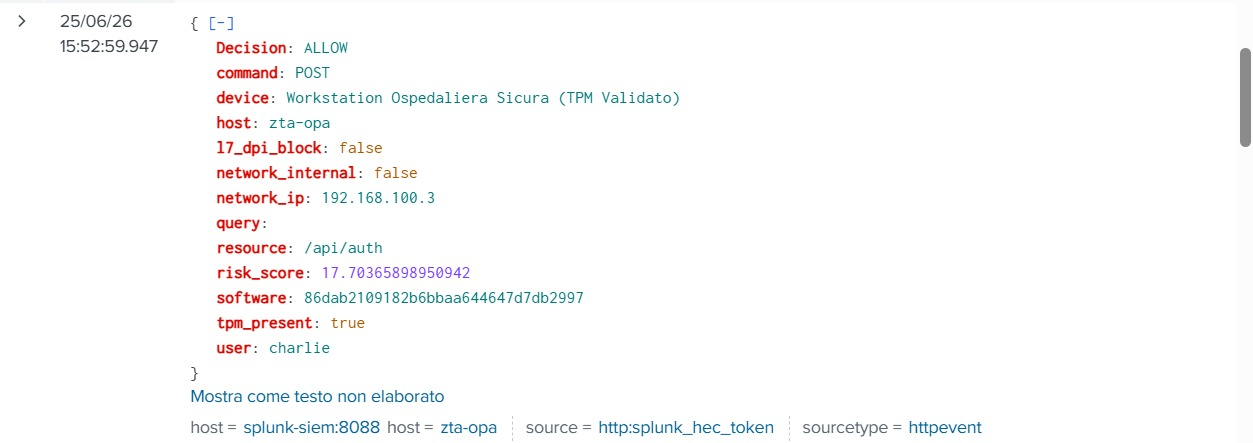
\includegraphics[width=0.9\linewidth]{capitolo4/img/splunk_charlie_allowed.jpeg}
    \caption{Log di autorizzazione (ALLOW) per Charlie: il verdetto è positivo nonostante la rete esterna (\texttt{network\_internal: false}), grazie al basso \textit{risk\_score} ($17.7 \le 26$).}
    \label{fig:splunk_charlie_allowed}
\end{figure}

\begin{figure}[H]
\centering
\resizebox{0.75\linewidth}{!}{%
\begin{tikzpicture}[
    zonebox/.style 2 args={
        fill=#1!15!darkcharcoal, draw=#1, solid, line width=1.2pt,
        rounded corners=6pt, inner sep=12pt,
        label={[font=\footnotesize\bfseries\sffamily, text=#1]#2}
    },
    untrustedbox/.style={draw=copper, fill=copper!8!darkcharcoal, text=cream, rounded corners=3pt,
        minimum width=2.0cm, minimum height=1.5cm, align=center, font=\scriptsize\sffamily,
        drop shadow={opacity=0.12, color=black}},
    fwbox/.style={draw=copper, fill=copper!8!darkcharcoal, text=cream, rounded corners=3pt,
        minimum width=2.2cm, minimum height=1.5cm, align=center, font=\scriptsize\sffamily,
        drop shadow={opacity=0.12, color=black}},
    pepbox/.style={draw=green!60!black, fill=green!60!black, text=white, rounded corners=4pt,
        minimum width=2.2cm, minimum height=1.5cm, align=center, font=\scriptsize\bfseries\sffamily,
        drop shadow={opacity=0.18, color=black}},
    corebox/.style={draw=sand, fill=sand!8!darkcharcoal, text=cream, rounded corners=3pt,
        minimum width=2.2cm, minimum height=1.5cm, align=center, font=\scriptsize\sffamily},
    controlbox/.style={draw=textmuted, fill=textmuted!8!darkcharcoal, text=cream, rounded corners=3pt,
        minimum width=2.2cm, minimum height=1.5cm, align=center, font=\scriptsize\sffamily},
    arr/.style={-{Stealth[scale=0.8]}, draw=copper, line width=1pt},
    passarr/.style={-{Stealth[scale=0.85]}, draw=green!70!black, line width=1.5pt},
    darr/.style={-{Stealth[scale=0.7]}, draw=textmuted, densely dashed, line width=0.7pt},
    lbl/.style={font=\tiny\bfseries\sffamily}
]
    \node[untrustedbox, draw=copper, line width=2pt] (charlie) at (2, 0) {\textbf{Charlie (Remote)}};
    \node[fwbox] (fw) at (6, 0) {Firewall};
    \node[pepbox, draw=green!60!black, line width=2pt] (pep) at (10, 0) {Envoy (PEP)};
    \node[corebox] (webapi) at (14, 0) {Web API};
    \node[controlbox] (opa) at (12, -5) {\textbf{OPA}};
    \node[controlbox] (splunk) at (8, -5) {\textbf{Splunk ML}};

    \draw[passarr] (charlie.east) -- (fw.west);
    \draw[passarr] (fw.east) -- (pep.west);
    \draw[passarr] (pep.east) -- node[above, lbl]{ALLOW} (webapi.west);
    \draw[arr] (pep.south) -- (opa.north);
    \draw[arr] (opa.west) -- (splunk.east);
    \node[below=0.02cm of pep, font=\scriptsize\bfseries\sffamily\color{green!60!black}] {VERDETTO: ALLOW};
\end{tikzpicture}%
}
\caption{Mappatura logica dei flussi nello Scenario 6 (Accesso autorizzato per rischio contenuto).}
\label{fig:scenario_charlie}
\end{figure}

\subsection{Scenario 7: Accesso ai dati sensibili: Alice (utente interno)}
Questo scenario illustra la capacità del sistema di implementare politiche di autorizzazione contestuali basate sulla sensibilità della risorsa target. Alice, medico con credenziali valide e workstation certificata (TPM), tenta l'accesso al \textit{Fascicolo Sanitario Elettronico} di un paziente, che contiene dati clinici riservati.

A differenza dell'accesso alla dashboard principale, l'apertura del fascicolo attiva una richiesta specifica verso l'endpoint \texttt{/api/patients/sensitive}. OPA valuta la richiesta considerando non solo le dimensioni contestuali (identità, dispositivo, rete), ma anche il parametro \texttt{sensitivity\_level} della risorsa richiesta. Come mostrato in Figura~\ref{fig:alice_notes}, il sistema autorizza la visualizzazione delle note sensibili (es. patologie infettive e protocolli di rischio biologico) unicamente in presenza di un contesto di sicurezza totale: workstation interna, TPM validato e assenza di anomalie comportamentali.

\begin{figure}[H]
    \centering
    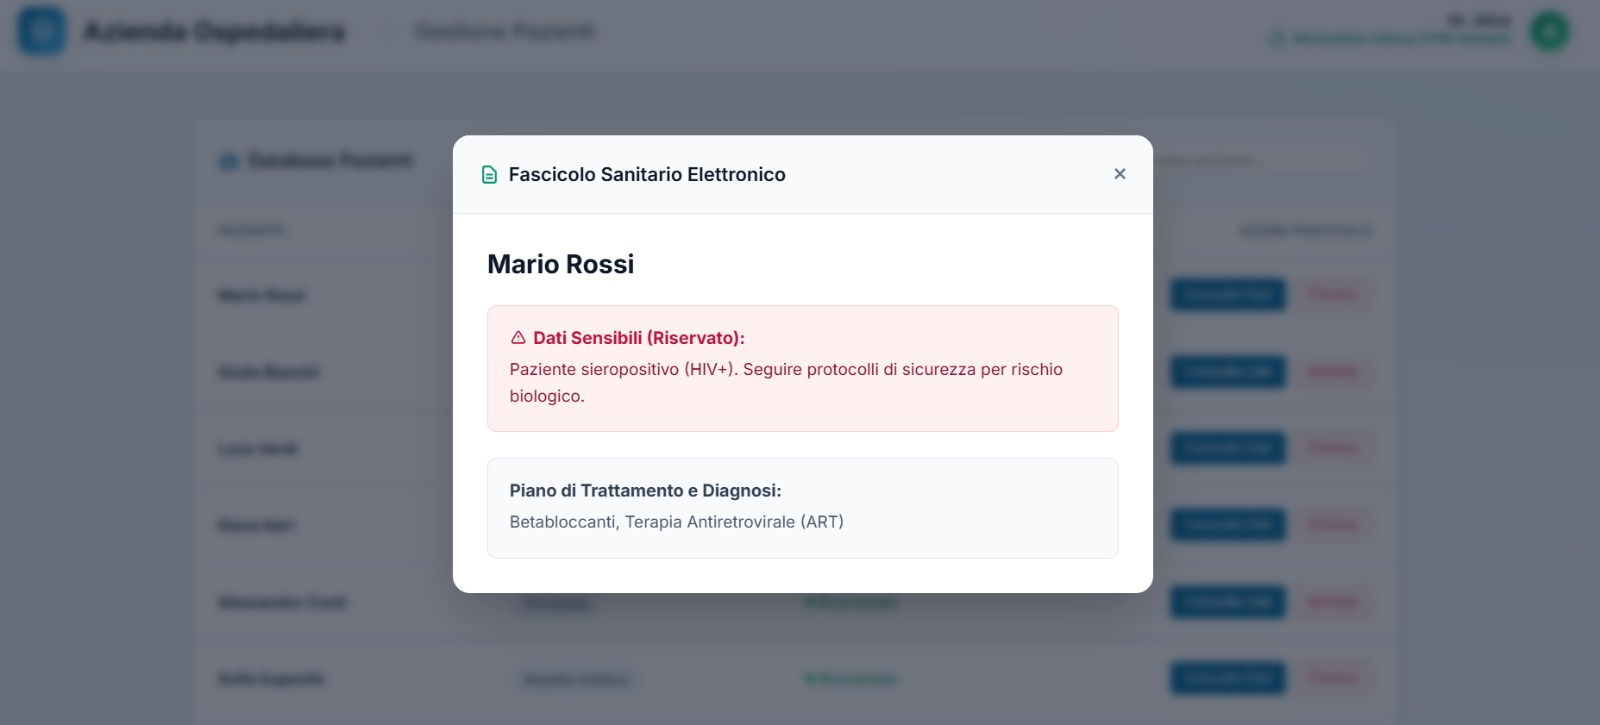
\includegraphics[width=0.9\textwidth]{capitolo4/img/alice_notes.jpeg}
    \caption{Visualizzazione autorizzata del Fascicolo Sanitario Elettronico contenente dati sensibili da parte di Alice.}
    \label{fig:alice_notes}
\end{figure}

L'architettura applica qui il principio di \textit{Least Privilege}: qualora uno qualsiasi dei parametri di sicurezza risultasse alterato — ad esempio, se Alice tentasse di accedere a queste stesse informazioni collegandosi dalla rete esterna — la richiesta verrebbe negata dal PEP, nonostante la validità dell'identità dell'utente. Il sistema garantisce così che il trattamento di dati particolarmente protetti sia confinato entro il perimetro di massima sicurezza dell'ospedale, prevenendo l'esposizione di informazioni sanitarie sensibili in ambienti potenzialmente esposti a intercettazioni o accessi non autorizzati.

\subsection{Scenario 8: Accesso ai dati sensibili: Charlie (utente remoto)}
Questo scenario valida la capacità del sistema di negare l'accesso a informazioni critiche basandosi su una valutazione contestuale, anche in presenza di un utente e di un dispositivo pienamente conformi. Charlie, operatore remoto con attestazione hardware (TPM) valida, tenta di accedere alle note sensibili dei pazienti (\texttt{/api/patients/sensitive}).

Nonostante l'autenticazione sia avvenuta correttamente nello Scenario 6, OPA intercetta la richiesta verso l'endpoint sensibile ed esegue una \textit{Deep Packet Inspection} (DPI) applicativa. Rilevando che il parametro \texttt{network\_internal} è impostato su \texttt{false}, OPA impone il blocco dell'operazione per prevenire l'esposizione di dati clinici riservati fuori dal perimetro di rete protetto, come illustrato nella Figura~\ref{fig:charlie_notes}.

\begin{figure}[H]
    \centering
    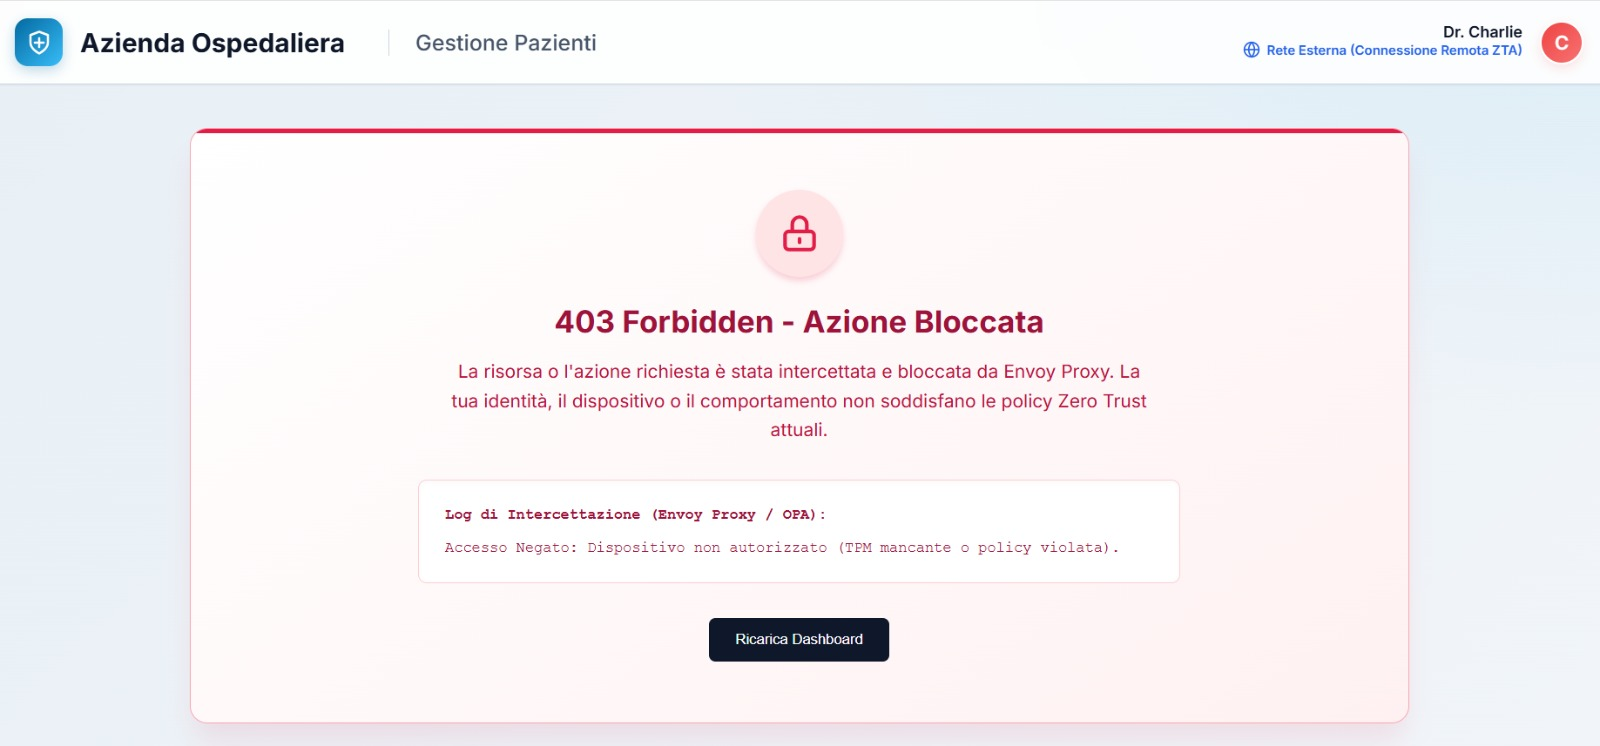
\includegraphics[width=0.9\textwidth]{capitolo4/img/charlie_notes.jpeg}
    \caption{Pagina di blocco 403 Forbidden visualizzata da Charlie nel tentativo di accedere ai dati sensibili da remoto.}
    \label{fig:charlie_notes}
\end{figure}

Il log di Splunk in Figura~\ref{fig:splunk_charlie_notes} documenta la decisione di \textbf{DENY}: il campo \texttt{l7\_dpi\_block} è impostato su \texttt{true}, confermando che il blocco è stato applicato a livello L7 dal proxy Envoy su indicazione di OPA.

\begin{figure}[H]
    \centering
    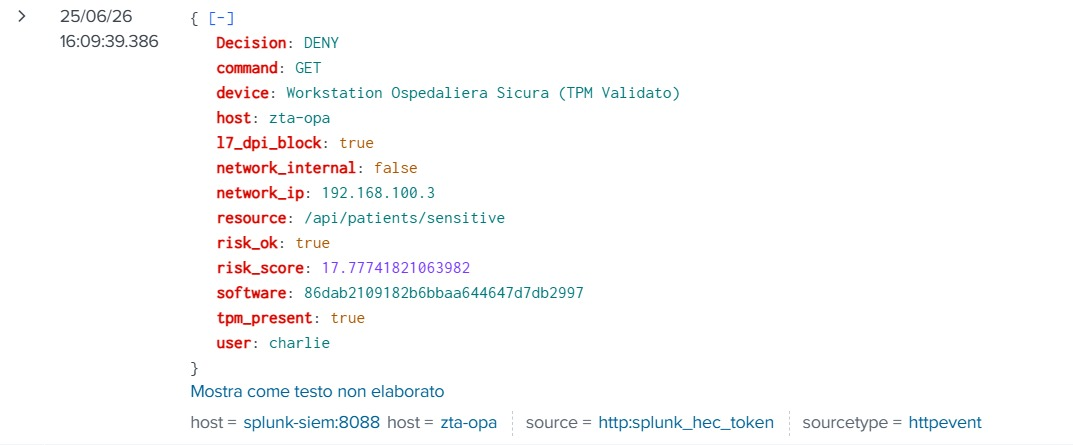
\includegraphics[width=0.95\textwidth]{capitolo4/img/splunk_charlie_notes.jpeg}
    \caption{Log di blocco (DENY) per l'accesso ai dati sensibili di Charlie: il sistema applica il blocco DPI (\texttt{l7\_dpi\_block: true}) a causa della rete esterna.}
    \label{fig:splunk_charlie_notes}
\end{figure}

Questo scenario è fondamentale per confermare l'efficacia del modello \textit{Defense in Depth}: il sistema non si accontenta di una sessione autenticata, ma esegue una \textit{Continuous Authorization} per ogni singola risorsa richiesta. Il diniego non è dovuto a una mancanza di permessi dell'utente, bensì alla protezione intrinseca del dato sensibile, che richiede — per policy — una connessione dalla rete interna aziendale per essere visualizzato.

\subsection{Scenario 9: Protezione dell'accesso TCP diretto}
Il nono scenario ha lo scopo di validare la coerenza e l'impermeabilità delle policy Zero Trust anche sui canali di comunicazione di livello trasporto (Layer 4). Nello specifico, si intende dimostrare che il proxy Envoy, operante come \textit{TCP Proxy} sulla porta nativa del database (27017), impone le medesime restrizioni di identità e \textit{Device Posture} già verificate per il traffico Web HTTP, impedendo \textit{bypass} architetturali.

Viene inizialmente condotto un test di connessione diretta (tramite driver \texttt{pymongo}) da parte di Alice, utente legittimo provvisto di dispositivo conforme:

\begin{center}
\begin{minipage}{\linewidth}
\begin{ztacodebox}{pymongo\_alice\_tcp.sh}
\begin{lstlisting}[language=bash]
$ docker exec -it zta-client-alice python3 -c "import pymongo; \
  client = pymongo.MongoClient('zta-envoy', 27017, tls=True, \
  tlsCertificateKeyFile='/etc/certs/alice_combined.pem', \
  tlsCAFile='/etc/certs/ca.crt', tlsAllowInvalidHostnames=True, \
  serverSelectionTimeoutMS=10000); db = client['hospital_db']; \
  print('Risultato:', db.command('ping'))"
Risultato: {'ok': 1.0}
\end{lstlisting}
\end{ztacodebox}
\captionof{lstlisting}{Connessione TCP al database autorizzata per dispositivo conforme (Alice).}\label{lst:pymongo_alice_tcp}
\end{minipage}
\end{center}

Come mostrato nel Listato~\ref{lst:pymongo_alice_tcp}, il filtro di rete \texttt{ext\_authz} intercetta il tentativo di instaurazione del \textit{socket}. OPA analizza i metadati crittografici, rileva la presenza dell'estensione hardware TPM (\texttt{tpm\_present: true}) ed autorizza l'apertura del tunnel TCP bidirezionale, permettendo al comando di \textit{ping} di raggiungere la risorsa.

Il secondo test speculare viene eseguito da Bob, dotato di credenziali legittime ma operante su un computer personale sprovvisto di modulo TPM:

\begin{center}
\begin{minipage}{\linewidth}
\begin{ztacodebox}{pymongo\_bob\_tcp.sh}
\begin{lstlisting}[language=bash]
$ docker exec -it zta-client-bob python3 -c "import pymongo; \
  client = pymongo.MongoClient('zta-envoy', 27017, tls=True, \
  tlsCertificateKeyFile='/etc/certs/bob_combined.pem', \
  tlsCAFile='/etc/certs/ca.crt', tlsAllowInvalidHostnames=True, \
  serverSelectionTimeoutMS=10000); db = client['hospital_db']; \
  print('Risultato:', db.command('ping'))"
pymongo.errors.ServerSelectionTimeoutError: zta-envoy:27017: connection closed
\end{lstlisting}
\end{ztacodebox}
\captionof{lstlisting}{Tentativo di connessione TCP abortito per dispositivo non conforme (Bob).}\label{lst:pymongo_bob_tcp}
\end{minipage}
\end{center}

Il Listato~\ref{lst:pymongo_bob_tcp} evidenzia l'efficacia del blocco preventivo. OPA nega l'autorizzazione alla radice (\textbf{DENY}) per via della mancata conformità hardware; Envoy applica immediatamente il verdetto interrompendo la negoziazione (\texttt{connection closed}) ed impedendo fisicamente la creazione del tunnel TCP.

Questo risultato finale attesta che la microsegmentazione Zero Trust risulta coerente su tutta l'architettura: il database è protetto a livello di trasporto (\textit{Layer 4}) in modo identico alle \textit{Web API} (\textit{Layer 7}), garantendo che le risorse critiche siano invisibili e irraggiungibili per qualsiasi \textit{endpoint} non pienamente fidato.

\subsection{Scenario 10: Protezione dai payload dannosi a livello applicativo (L7)}
Questo scenario valida la capacità del sistema di operare una \textit{Deep Packet Inspection} (DPI) applicativa. Anche un utente legittimo come Alice, in possesso di un dispositivo conforme e attestazione TPM valida, viene bloccato qualora tenti di eseguire operazioni non permesse dalle policy di sicurezza, come la cancellazione di dati clinici.

L'attacco viene simulato tramite l'invio di una richiesta HTTP con metodo \texttt{DELETE} verso l'endpoint \texttt{/api/patients}. Come mostrato in Figura~\ref{fig:alice_delete_ui}, il sistema non solo rifiuta l'operazione, ma fornisce un feedback immediato all'utente tramite una pagina di blocco dedicata, specificando che l'azione viola le policy Zero Trust.

\begin{figure}[H]
    \centering
    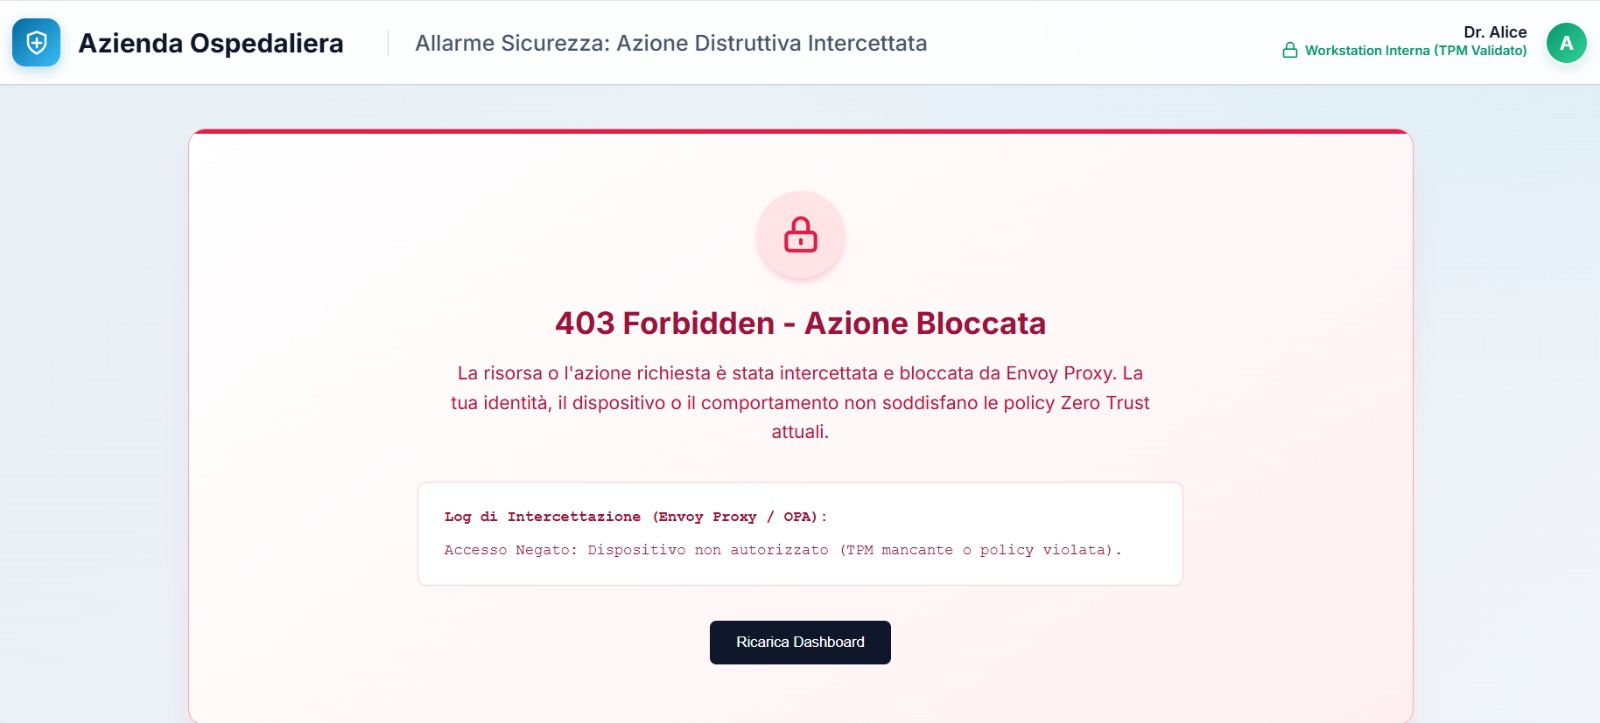
\includegraphics[width=0.9\textwidth]{capitolo4/img/delete.jpeg}
    \caption{Interfaccia di blocco visualizzata da Alice a seguito del tentativo di esecuzione di metodo \texttt{DELETE}.}
    \label{fig:alice_delete_ui}
\end{figure}

Dal punto di vista dell'architettura di controllo, l'intercettazione avviene a livello di proxy Envoy prima che la richiesta possa raggiungere il database. Il sistema registra l'evento in Splunk in tempo reale, permettendo al team di sicurezza di analizzare il tentativo di violazione con estrema granularità:

\begin{figure}[H]
    \centering
    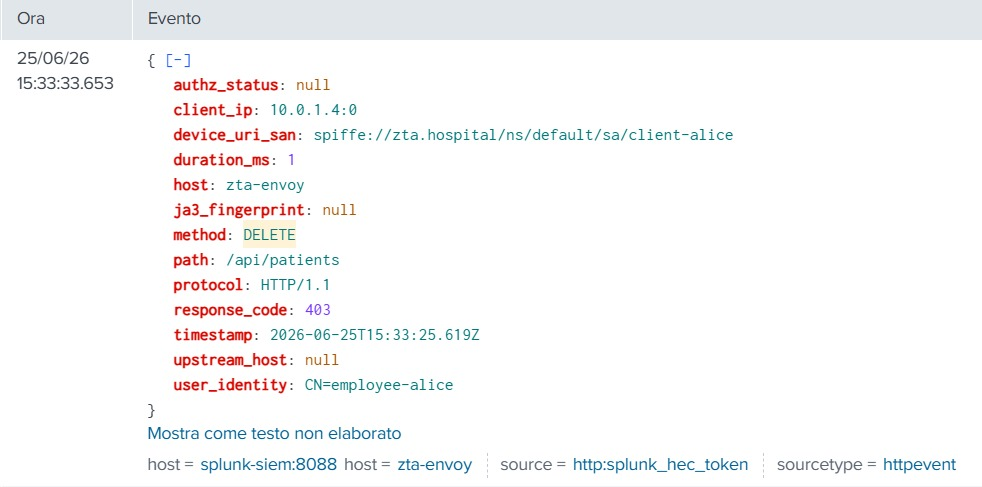
\includegraphics[width=0.95\textwidth]{capitolo4/img/log_delete.jpeg}
    \caption{Log dell'evento di blocco indicizzato in Splunk: evidenza dell'operazione \texttt{DELETE} respinta.}
    \label{fig:alice_delete_log}
\end{figure}

Come si evince dal log in Figura~\ref{fig:alice_delete_log}, il campo \texttt{method} riporta chiaramente l'operazione \texttt{DELETE}, mentre il \texttt{response\_code} a \texttt{403} conferma l'avvenuto blocco. Questo scenario dimostra l'efficacia della microsegmentazione applicativa: il sistema agisce come un \textit{Web Application Firewall} (WAF) consapevole del contesto, in cui le autorizzazioni non sono solo basate sull'identità dell'utente, ma sul principio del \textit{Least Privilege} applicato ai verbi HTTP e alle operazioni sui dati. Il medesimo meccanismo di DPI si applica anche alle connessioni dirette al database MongoDB (porta \texttt{27017}): in quel caso il blocco è delegato ad OPA tramite il filtro \texttt{mongo\_proxy}, con il modello Splunk MLTK che calcola il risk score prima dell'enforcement finale.

\subsubsection{Simulazione di compromissione del dispositivo e blocco comportamentale}
\label{sec:compromissione}

Si analizza infine lo scenario più critico previsto dal framework Zero Trust: la compromissione totale della postazione di un utente legittimo (\textit{Insider Threat} o furto fisico). In questo scenario, l'attaccante dispone del dispositivo di Alice, del chip TPM validato e di tutti i certificati mTLS necessari. L'obiettivo dell'attaccante è bypassare i controlli applicativi di livello 7 (le Web API) e connettersi direttamente al database MongoDB attraverso la porta TCP nativa \texttt{27017}.

Per gestire minacce di questa natura, l'architettura non si affida esclusivamente ai controlli statici al perimetro, ma implementa all'interno del \textit{Policy Information Point} (PIP) un sistema di tracciamento comportamentale \textit{in-memory}. 

\begin{center}
\begin{minipage}{\linewidth}
\begin{ztacodebox}{pip\_behavioral\_tracker.py (Estratto Essenziale)}
\begin{lstlisting}[language=Python]
# Tracker comportamentali in-memory (TTL-based eviction)
failed_login_tracker = defaultdict(list)
session_tracker = defaultdict(list)

def enrich_spl_with_behavioral_features(query: str) -> str:
    user = extract_user_from_spl(query)
    resource = extract_resource_from_spl(query)
    
    # Rilevamento connessione diretta al DB (Simulazione PC compromesso)
    is_compromised_alice = (user == "alice" and "MongoDB" in resource)

    if is_compromised_alice:
        # Iniezione anomalie gravissime (device theft / insider threat)
        failed_logins, session_freq, days_inactive = 4, 30, 60
        is_night, hour_of_day = 1, 3
    else:
        # Flusso utente standard (lettura dati reali)
        failed_logins = len(failed_login_tracker[user])
        session_freq = len(session_tracker[user])
        days_inactive, is_night, hour_of_day = 0, 0, datetime.now().hour

    # Costruzione delle feature aggiuntive
    features = (
        f', failed_logins={failed_logins}, session_freq={session_freq}'
        f', days_inactive={days_inactive}, is_night={is_night}'
        f', hour_of_day={hour_of_day}, sensitivity_level=3'
    )

    # Inietta le feature prima del comando '| apply' di Splunk
    return query.replace('| apply ', f'{features} | apply ')
\end{lstlisting}
\end{ztacodebox}
\captionof{lstlisting}{Estratto della logica di arricchimento comportamentale nel PIP.}\label{lst:pip_behavioral}
\end{minipage}
\end{center}

Come si evince dal Listato~\ref{lst:pip_behavioral}, il PIP funge da mediatore intelligente: non si limita a inoltrare la richiesta ad OPA, ma mantiene uno stato storico delle sessioni tramite dizionari aggiornati in tempo reale. Quando la funzione \texttt{enrich\_spl\_with\_behavioral\_features} intercetta la query destinata al modello di Machine Learning, vi inietta le variabili comportamentali dell'utente. Nel caso specifico della simulazione di attacco (\texttt{is\_compromised\_alice}), il codice inietta deliberatamente metriche fortemente degradate — quali 60 giorni di inattività pregressa, un'anomala frequenza di sessione e un orario notturno — per istruire il modello MLTK sulla presenza di un probabile furto di credenziali o dispositivo.

Per innescare concretamente questa logica difensiva, si esegue dal terminale del container di Alice uno script Python che tenta l'instaurazione del \textit{socket} TCP:

\begin{center}
\begin{minipage}{\linewidth}
\begin{ztacodebox}{alice\_bypass\_mongodb.py}
\begin{lstlisting}[language=Python]
$ docker exec zta-client-alice python3 -c "
import pymongo
client = pymongo.MongoClient(
    'zta-envoy', 27017,
    tls=True,
    tlsCertificateKeyFile='/etc/certs/alice_combined.pem',
    tlsCAFile='/etc/certs/ca.crt',
    tlsAllowInvalidHostnames=True,
    serverSelectionTimeoutMS=10000
)
db = client['hospital_db']
result = list(db.patients.find({'sensitive_notes': 'test'}))
"
\end{lstlisting}
\end{ztacodebox}
\captionof{lstlisting}{Simulazione di accesso diretto al database MongoDB dal dispositivo compromesso di Alice.}\label{lst:alice_bypass_mongodb}
\end{minipage}
\end{center}

Il Listato~\ref{lst:alice_bypass_mongodb} illustra la gravità della minaccia: lo script sfrutta la libreria \texttt{pymongo} passando esplicitamente i certificati crittografici legittimi (\texttt{alice\_combined.pem} e \texttt{ca.crt}). Questo garantisce il superamento indolore dell'handshake mTLS imposto da Envoy. Senza un'analisi comportamentale di livello superiore, questa connessione verrebbe considerata perfettamente autorizzata da qualsiasi firewall tradizionale.

Il sistema di tracciamento (Listato~\ref{lst:pip_behavioral}) interviene marcando la richiesta come altamente anomala: l'identità di Alice presenta storicamente 60 giorni di inattività e 4 tentativi di login pregressi falliti in rapida successione. L'arricchimento della query SPL con queste feature fa sì che il modello predittivo restituisca un punteggio di rischio pari a $\approx 95.49$. Poiché tale valore supera ampiamente la soglia di tolleranza massima di $38$ impostata in OPA per gli utenti interni, la policy emette un verdetto di \textbf{DENY}. Envoy chiude brutalmente il \textit{socket} TCP, impedendo la connessione.

La Figura~\ref{fig:splunk_alice_bypass_deny} mostra il log di decisione indicizzato in Splunk. È fondamentale notare come il sistema riconosca l'identità corretta (\texttt{user: alice}), confermi la validità dell'hardware (\texttt{tpm\_present: true}) e della rete (\texttt{network\_internal: true}), ma blocchi l'accesso unicamente a causa della metrica comportamentale (\texttt{risk\_ok: false}).

\begin{figure}[H]
\centering
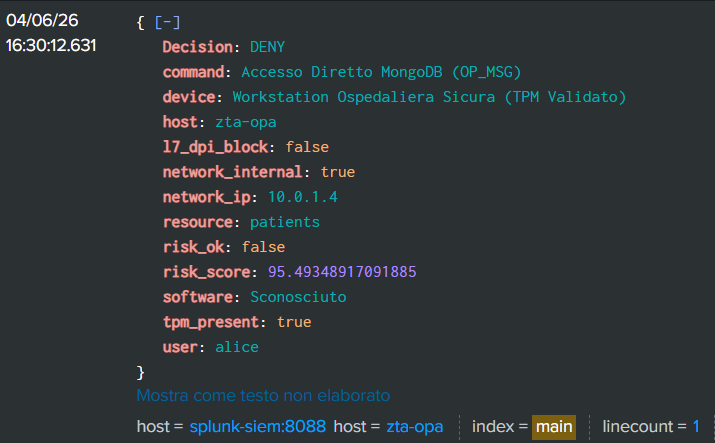
\includegraphics[width=0.9\linewidth]{capitolo4/img/splunk_alice_bypass_deny.png}
\caption{Log di decisione DENY indicizzato in Splunk: l'accesso diretto viene bloccato nonostante la validità crittografica, a causa del rischio comportamentale estremo ($95.49 > 38$).}
\label{fig:splunk_alice_bypass_deny}
\end{figure}

Questo test dimostra l'assunto cardine della \textit{Continuous Authorization} Zero Trust: l'autenticazione crittografica forte non è mai sufficiente da sola. Anche il dispositivo più sicuro viene disconnesso dalla rete nel momento in cui l'analisi euristica ne identifica un pattern di utilizzo incompatibile con la normale operatività dell'utente.

\begin{figure}[H]
\centering
\resizebox{0.75\linewidth}{!}{%
\begin{tikzpicture}[
    zonebox/.style 2 args={
        fill=#1!15!darkcharcoal, draw=#1, solid, line width=1.2pt,
        rounded corners=6pt, inner sep=12pt,
        label={[font=\footnotesize\bfseries\sffamily, text=#1]#2}
    },
    untrustedbox/.style={draw=copper, fill=copper!8!darkcharcoal, text=cream, rounded corners=3pt,
        minimum width=2.0cm, minimum height=1.5cm, align=center, font=\scriptsize\sffamily,
        drop shadow={opacity=0.12, color=black}},
    dmzbox/.style={draw=terracotta, fill=terracotta!8!darkcharcoal, text=cream, rounded corners=3pt,
        minimum width=2.0cm, minimum height=1.5cm, align=center, font=\scriptsize\sffamily,
        drop shadow={opacity=0.12, color=black}},
    fwbox/.style={draw=copper, fill=copper!8!darkcharcoal, text=cream, rounded corners=3pt,
        minimum width=2.2cm, minimum height=1.5cm, align=center, font=\scriptsize\sffamily,
        drop shadow={opacity=0.12, color=black}},
    corebox/.style={draw=sand, fill=sand!8!darkcharcoal, text=cream, rounded corners=3pt,
        minimum width=2.2cm, minimum height=1.5cm, align=center, font=\scriptsize\sffamily,
        drop shadow={opacity=0.12, color=black}},
    controlbox/.style={draw=textmuted, fill=textmuted!8!darkcharcoal, text=cream, rounded corners=3pt,
        minimum width=2.2cm, minimum height=1.5cm, align=center, font=\scriptsize\sffamily,
        drop shadow={opacity=0.12, color=black}},
    pepbox/.style={draw=copper, fill=copper, text=white, rounded corners=4pt,
        minimum width=2.2cm, minimum height=1.5cm, align=center, font=\scriptsize\bfseries\sffamily,
        drop shadow={opacity=0.18, color=black}},
    arr/.style={-{Stealth[scale=0.8]}, draw=copper, line width=1pt},
    successarr/.style={-{Stealth[scale=0.85]}, draw=green!70!black, line width=1.5pt},
    failarr/.style={-{Stealth[scale=0.85]}, draw=red!70!black, line width=1.5pt},
    blockarr/.style={-{Stealth[scale=0.7]}, draw=red!60!black, line width=1.5pt, dashed},
    darr/.style={-{Stealth[scale=0.7]}, draw=textmuted, densely dashed, line width=0.7pt},
    lbl/.style={font=\tiny\bfseries\sffamily}
]

    \node[untrustedbox, draw=textmuted, text=textmuted] (charlie) at (2, 2.2)
        {
\includegraphics[height=0.55cm]{capitolo2/img/charlie.png}\\[0.05cm]\textbf{Charlie}};
    \node[dmzbox, draw=green!80!black, line width=2pt] (alice) at (2, 0)
        {
\includegraphics[height=0.55cm]{capitolo2/img/alice.png}\\[0.05cm]\textbf{Alice (Compromessa)}};
    \node[dmzbox, draw=textmuted, text=textmuted] (bob)   at (2,-2)
        {
\includegraphics[height=0.55cm]{capitolo2/img/bob.png}\\[0.05cm]\textbf{Bob}};
    \node[fwbox, draw=green!80!black, line width=1.5pt]   (fw)    at (6, 0)
        {
\includegraphics[width=0.7cm]{capitolo2/img/nftables.png}\\[0.03cm]\textbf{Firewall}};
    \node[pepbox, draw=red!80!black, line width=2pt] (pep) at (10, 0)
        {
\includegraphics[width=0.7cm]{capitolo2/img/envoy.png}\\[0.03cm]Envoy};
    \node[corebox, draw=green!80!black, line width=1.5pt] (webapi)  at (14, 1.2)
        {
\includegraphics[width=0.7cm]{capitolo2/img/python.png}\\[0.03cm]\textbf{Web API (PIP)}};
    \node[corebox, draw=red!80!black, line width=1.5pt] (mongodb) at (14,-1.2)
        {
\includegraphics[width=0.7cm]{capitolo2/img/mongodb.png}\\[0.03cm]\textbf{MongoDB}};
    \node[controlbox] (snort) at (3.5, -5)
        {
\includegraphics[width=0.7cm]{capitolo2/img/snort.png}\\[0.03cm]\textbf{Snort}};
    \node[controlbox, draw=red!80!black, line width=1.5pt] (splunk) at (3.5, -7.5)
        {
\includegraphics[width=0.7cm]{capitolo2/img/splunk.png}\\[0.03cm]\textbf{Splunk MLTK}};
    \node[controlbox] (fluentbit) at (8, -7.5)
        {
\includegraphics[width=0.7cm]{capitolo2/img/fluentbit.png}\\[0.03cm]\textbf{Fluent-Bit}};
    \node[controlbox, draw=red!80!black, line width=1.5pt] (opa) at (12.5, -7.5)
        {
\includegraphics[width=0.7cm]{capitolo2/img/opa.png}\\[0.03cm]\textbf{OPA}};

    \node[below=0.02cm of alice, font=\scriptsize\bfseries\sffamily\color{green!80!black}] {mTLS+TPM Validi};
    \node[above=0.02cm of pep, font=\scriptsize\bfseries\sffamily\color{red!80!black}] {DENY: Rischio ML Anomalo};
    \node[below=0.02cm of mongodb, font=\scriptsize\bfseries\sffamily\color{red!80!black}] {TCP Bloccato};
    \node[below=0.02cm of splunk, font=\scriptsize\bfseries\sffamily\color{red!80!black}] {Score 95.49};
    \node[below=0.02cm of opa, font=\scriptsize\bfseries\sffamily\color{red!80!black}] {risk\_score > 50};

    \begin{scope}[on background layer]
        \node[zonebox={copper}{above:Rete Esterna}, inner sep=7pt]          [fit=(charlie)] {};
        \node[zonebox={terracotta}{below:Rete Interna}, inner sep=7pt]  [fit=(alice)(bob)] {};
        \node[zonebox={sand}{above:Risorse Protette}]           [fit=(webapi)(mongodb)] {};
        \node[zonebox={textmuted}{below:Piano di Controllo}]    [fit=(opa)(fluentbit)(splunk)] {};
    \end{scope}

    \draw[successarr] (alice.east)   -- node[above, lbl, pos=0.5, color=terracotta]{mTLS+TPM} (fw.west);
    \draw[successarr] (fw.east) -- node[above, lbl, color=copper]{DNAT} (pep.west);
    \draw[blockarr] (pep.east) -- node[right, lbl, color=red!80!black]{\textbf{BLOCCO TCP L4}} (mongodb.west);
    \draw[failarr] (pep.south) -- ++(0,-2.5) -| node[pos=0.2, above, lbl, color=red!70!black]{Verifica Authz} (opa.north);
    \draw[failarr] (opa.south) -- ++(0,-1.4) -| node[pos=0.5, above, lbl, color=red!70!black]{Query ML (tramite PIP)} (splunk.south);
    \draw[darr, draw=red!70!black] (pep.south)     to [bend left=10]  node[right, lbl, pos=0.6, color=red!70!black]{Log} (fluentbit.north);
    \draw[darr, draw=red!70!black] (fluentbit.west) -- node[above, lbl, color=red!70!black]{Inoltro Log} (splunk.east);

\end{tikzpicture}%
}
\caption{Mappatura logica dei flussi nello Scenario 10 (Blocco predittivo di una connessione per anomalie comportamentali, nonostante credenziali mTLS/TPM valide).}
\label{fig:scenario_l7_blocked}
\end{figure}

% ============================================================
% LAYER NIDS — MONITORAGGIO PERIMETRALE (Snort)
% ============================================================

\subsection{Scenario 11: Rilevamento di scansione di rete attiva (Nmap)}
Per validare l'efficacia del monitoraggio perimetrale, è stato condotto un test di ricognizione attiva mediante l'utility \texttt{nmap}, simulando un'attività di enumerazione dei servizi (\textit{service scanning}) da parte del nodo \textit{Charlie} verso il proxy \textit{Envoy}.

Il comando eseguito dal container di attacco è stato:
\begin{lstlisting}[language=bash, caption={Esecuzione di un service scan per mappare la superficie di attacco.}, label={lst:nmap_scan}]
docker exec -it zta-client-charlie nmap -sV zta-envoy
\end{lstlisting}

Il sistema IDS Snort, configurato in modalità passiva sul segmento di rete critico, ha immediatamente analizzato il traffico in transito. L'evento di scansione, identificato dalla regola \texttt{sid:1000001} (preposta al rilevamento di pattern di scansione SYN), è stato generato tempestivamente e inoltrato tramite Fluent-Bit al SIEM Splunk.

La Figura~\ref{fig:splunk_snort_nmap} mostra l'evidenza forense indicizzata: si nota come il sistema correli l'indirizzo sorgente dell'attaccante (\texttt{192.168.100.3}) con l'attività anomala verso il target protetto, permettendo al \textit{Security Operations Center} di visualizzare in tempo reale il tentativo di violazione.

\begin{figure}[htbp]
    \centering
    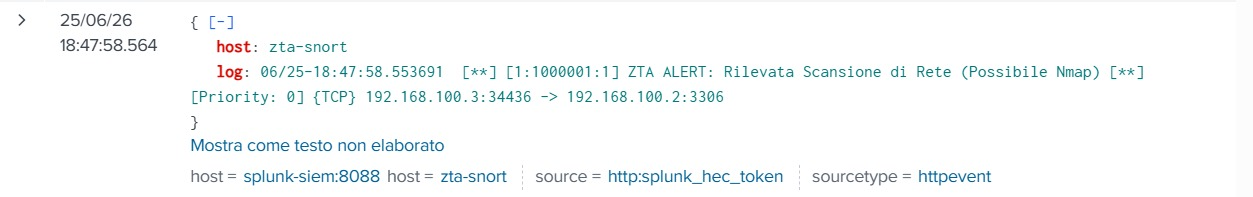
\includegraphics[width=0.95\linewidth]{capitolo4/img/nmap_snort.jpeg}
    \caption{Log di alert Snort (ZTA ALERT: Rilevata Scansione di Rete) centralizzato su Splunk, relativo allo scan Nmap eseguito da Charlie.}
    \label{fig:splunk_snort_nmap}
\end{figure}

L'integrazione tra l'IDS di rete e la piattaforma di analisi dei log dimostra la capacità del framework di non limitarsi alla sola protezione proattiva (tramite OPA/Envoy), ma di garantire una visibilità totale sulle minacce che tentano di mappare l'infrastruttura, chiudendo il ciclo di \textit{Detection \& Response}.

\subsection{Scenario 12: Audit delle connessioni native MongoDB}
Per verificare la capacità dell'infrastruttura di rilevare tentativi di accesso ai dati al di fuori delle Web API (protocollo nativo MongoDB), è stato eseguito un test di connessione diretta sulla porta \texttt{27017}. Tale scenario simula un attaccante che tenta di esfiltrare dati direttamente dal database, aggirando i controlli di livello applicativo.

Il comando di test, lanciato dal nodo di Charlie, è il seguente:
\begin{lstlisting}[language=bash, caption={Tentativo di connessione TCP diretta al database MongoDB.}, label={lst:mongo_test}]
docker exec -it zta-client-charlie bash -c "echo 'test' | nc zta-envoy 27017"
\end{lstlisting}

Snort, analizzando il traffico di rete, ha identificato il pacchetto TCP diretto alla porta standard del database e, in conformità con la regola \texttt{sid:1000002}, ha generato un alert di audit immediato. La Figura~\ref{fig:mongo_snort} mostra il log indicizzato in Splunk, che evidenzia la sorgente dell'attacco (\texttt{192.168.100.3}) e la destinazione (\texttt{192.168.100.2:27017}).

\begin{figure}[htbp]
    \centering
    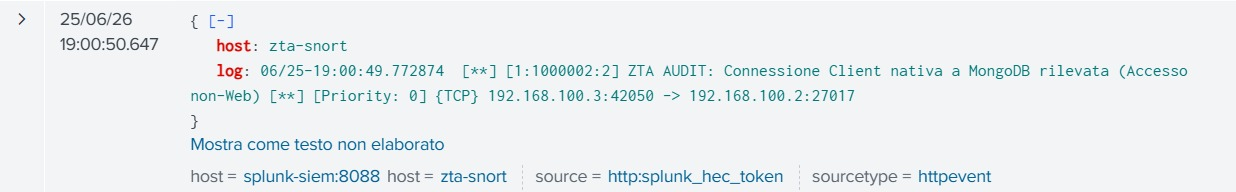
\includegraphics[width=0.95\linewidth]{capitolo4/img/mongo_snort.jpeg}
    \caption{Log di audit per connessione nativa a MongoDB non autorizzata.}
    \label{fig:mongo_snort}
\end{figure}

Questo riscontro conferma la validità del principio di \textit{Visibility} nel framework Zero Trust: anche quando un tentativo di intrusione non sfrutta vulnerabilità note, la semplice deviazione dal canale di comunicazione autorizzato (il traffico HTTPS verso le Web API) genera una traccia forense inequivocabile all'interno del SIEM, permettendo l'isolamento tempestivo del nodo malevolo.

\subsection{Scenario 13: Rilevamento di attacchi volumetrici (DoS)}
Per valutare la resilienza dell'infrastruttura di fronte a tentativi di saturazione delle risorse (Denial of Service), è stato simulato un attacco di tipo \textit{SYN Flood} verso l'endpoint \texttt{8443} del proxy \textit{Envoy}. Tale scenario mira a esaurire la tabella delle connessioni TCP attive, impedendo l'accesso agli utenti legittimi.

Il comando utilizzato per generare il carico volumetrico è stato:
\begin{lstlisting}[language=bash, caption={Generazione di traffico aggressivo per simulazione DoS.}, label={lst:dos_test}]
docker exec -it zta-client-charlie bash -c "for i in {1..150}; do nc -z -w1 zta-envoy 8443 & done; wait"
\end{lstlisting}

Il modulo IDS, configurato con una soglia di tolleranza di $100$ tentativi in $5$ secondi, ha prontamente intercettato l'anomalia. In conformità con la regola \texttt{sid:1000003}, il sistema ha generato un alert di priorità elevata, notificando tempestivamente il SIEM. La Figura~\ref{fig:snort_dos} illustra il log di allarme registrato su Splunk, che correla la sorgente dell'attacco con il tentativo di saturazione volumetrica del proxy.

\begin{figure}[htbp]
    \centering
    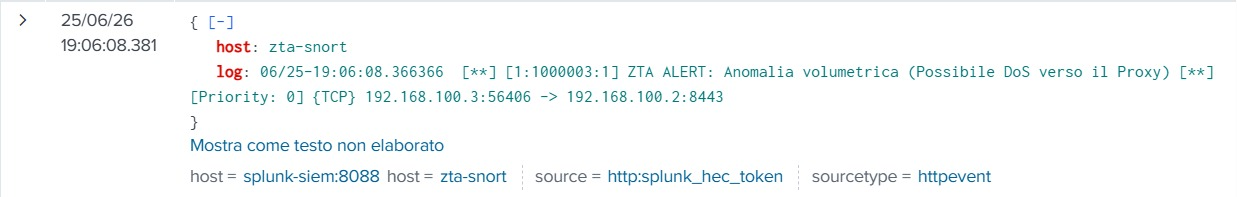
\includegraphics[width=0.95\linewidth]{capitolo4/img/snort_dos.jpeg}
    \caption{Log di alert Snort relativo all'anomalia volumetrica (DoS) verso il proxy Envoy.}
    \label{fig:snort_dos}
\end{figure}

Il tempestivo rilevamento conferma che il framework è in grado di distinguere tra un picco di traffico legittimo e un'attività malevola mirata alla compromissione della disponibilità del servizio. L'integrazione di tale metrica all'interno delle dashboard di \textit{Incident Response} consente, in uno scenario di produzione, l'attivazione di contromisure dinamiche, quali il \textit{rate-limiting} selettivo o l'inserimento in \textit{blacklist} temporanea dell'indirizzo IP aggressore mediante le policy del firewall di perimetro.

\subsection{Scenario 14: Rilevamento di attacchi di downgrade (traffico in chiaro)}
In un'architettura Zero Trust, la protezione della confidenzialità dei dati in transito è mandatoria. È stato quindi testato il comportamento del sistema di monitoraggio di fronte a un tentativo di \textit{Downgrade Attack}, dove un attaccante tenta di inviare richieste HTTP in chiaro verso la porta \texttt{8443}, nativamente protetta da TLS. L'obiettivo è verificare se l'IDS è in grado di identificare violazioni alla policy di crittografia end-to-end.

Il comando utilizzato per simulare l'invio del payload in chiaro è stato:
\begin{lstlisting}[language=bash, caption={Simulazione di richiesta HTTP in chiaro su porta protetta.}, label={lst:downgrade_test}]
docker exec -it zta-client-charlie bash -c "echo -e 'GET / HTTP/1.1\r\nHost: zta-envoy\r\n\r\n' | nc zta-envoy 8443"
\end{lstlisting}

Snort ha identificato la presenza della stringa \texttt{GET} all'interno del payload TCP diretto al proxy, attivando la regola \texttt{sid:1000004}. L'evento è stato immediatamente registrato e centralizzato nel SIEM, come documentato in Figura~\ref{fig:snort_http}.

\begin{figure}[htbp]
    \centering
    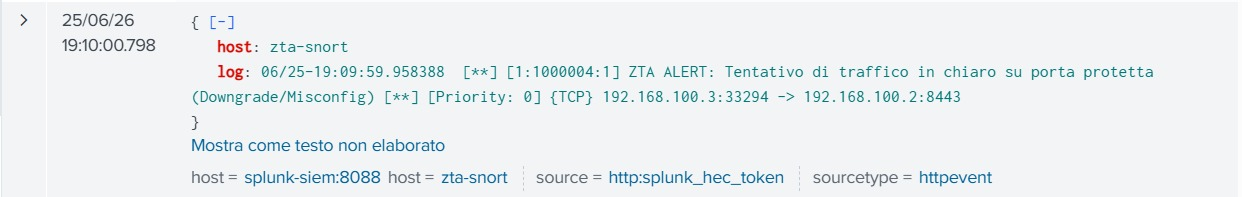
\includegraphics[width=0.95\linewidth]{capitolo4/img/snort_http.jpeg}
    \caption{Log di alert Snort relativo al rilevamento di traffico HTTP in chiaro su porta protetta (Downgrade).}
    \label{fig:snort_http}
\end{figure}

L'evidenza ottenuta dimostra l'efficacia del monitoraggio a livello pacchetto: mentre il proxy \textit{Envoy} agisce come \textit{enforcer} rifiutando la connessione, Snort funge da sensore per l'identificazione di tentativi di manomissione o misconfigurazioni, fornendo al SOC una notifica esplicita dell'intenzione malevola o del comportamento deviante rispetto agli standard di sicurezza definiti.

% ============================================================
% MONITORING — SPLUNK DASHBOARDS
% ============================================================

\subsection{Monitoraggio e Analisi in tempo reale: Splunk Dashboards}
Per garantire una visibilità end-to-end sull'infrastruttura e supportare le decisioni di sicurezza, sono state implementate specifiche dashboard di monitoraggio all'interno di Splunk. Queste interfacce non costituiscono semplici strumenti di visualizzazione, ma agiscono come veri e propri centri di comando per l'analisi comportamentale degli utenti e la gestione operativa degli incidenti in ottica Zero Trust.

La prima dashboard, denominata ``ZTA - Security Executive'' (Figura \ref{fig:dashboard1}), fornisce una visione d'insieme dello stato di salute del perimetro ospedaliero. Il \textit{Pannello A} offre una ripartizione statistica delle richieste processate dal sistema: il confronto tra \textit{Allow} e \textit{Deny} permette di validare in tempo reale l'efficacia delle policy di microsegmentazione attive. Il \textit{Pannello B} dettaglia il volume di traffico per singolo soggetto o dispositivo, consentendo di identificare rapidamente i nodi della rete con attività più intensa. Infine, il \textit{Pannello C} traccia la telemetria del traffico verso gli endpoint critici (\texttt{/api/auth}, \texttt{/api/patients}, \texttt{/api/patients/sensitive}), evidenziando picchi di carico che potrebbero sottendere tentativi di accesso massivo.

\begin{figure}[H]
    \centering
    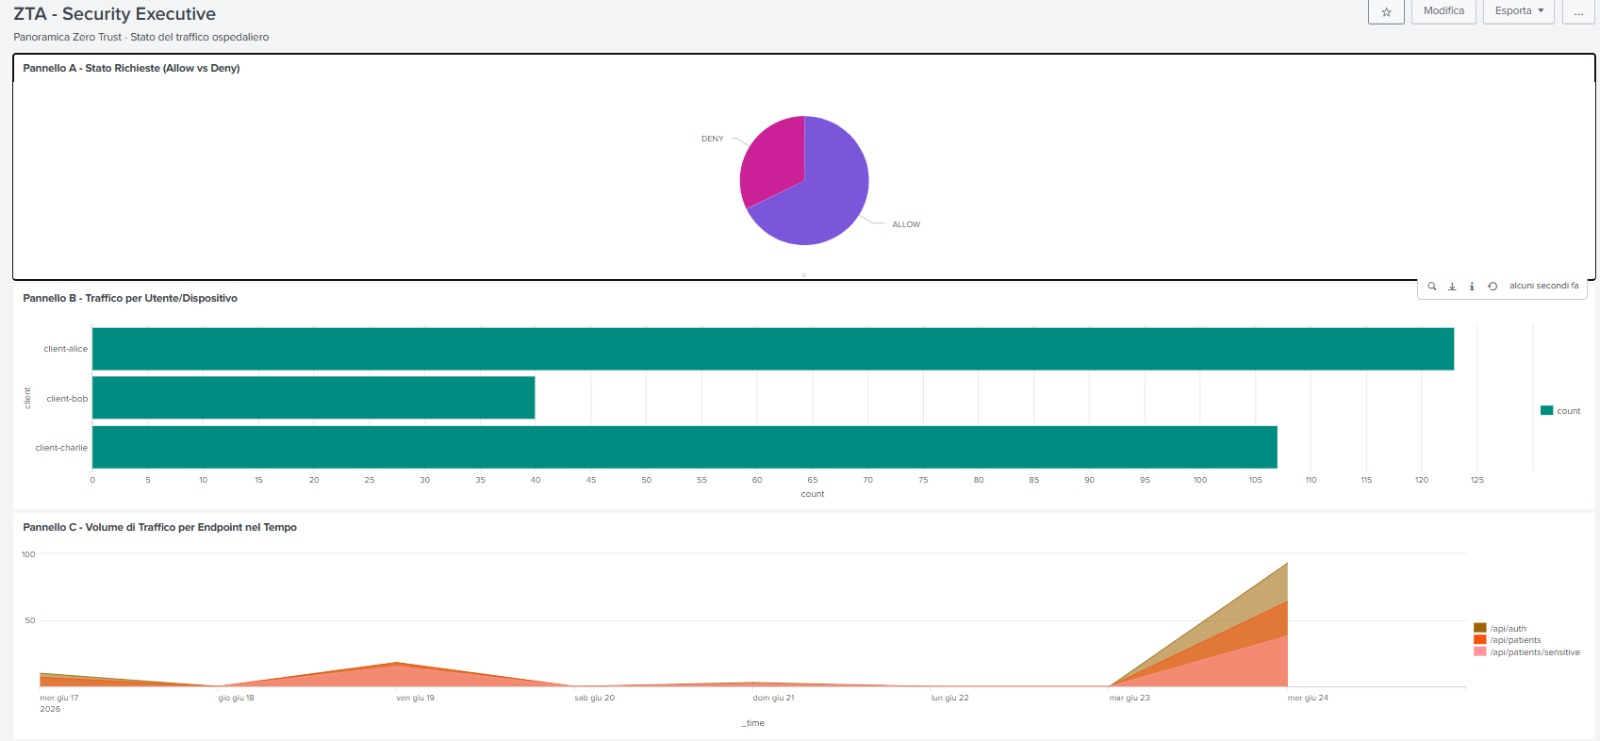
\includegraphics[width=1\textwidth]{capitolo4/img/dasboard1.jpeg}
    \caption{Dashboard ZTA - Security Executive: Panoramica e statistiche sul traffico.}
    \label{fig:dashboard1}
\end{figure}

Per la gestione attiva delle minacce, la dashboard ``ZTA - Incident Response'' (Figura \ref{fig:dashboard2}) centralizza le attività di contenimento. Il \textit{Pannello B} espone il conteggio aggregato delle richieste bloccate, rappresentando un KPI fondamentale per la valutazione del rischio residuo. Il \textit{Pannello A} fornisce l'evidenza forense delle violazioni L7 rilevate dal DPI: la tabella dettaglia il \textit{timestamp} preciso dell'attacco, l'identità del soggetto (\textit{user\_identity}), l'indirizzo IP, il metodo HTTP utilizzato e il \textit{path} tentato, mostrando chiaramente la decisione di \textit{BLOCKED} applicata dal PDP. Il \textit{Pannello C} correla le violazioni per indirizzo IP, evidenziando le sorgenti (es. \texttt{10.0.1.4} o \texttt{192.168.100.3}) che manifestano un comportamento malevolo ricorrente.

\begin{figure}[H]
    \centering
    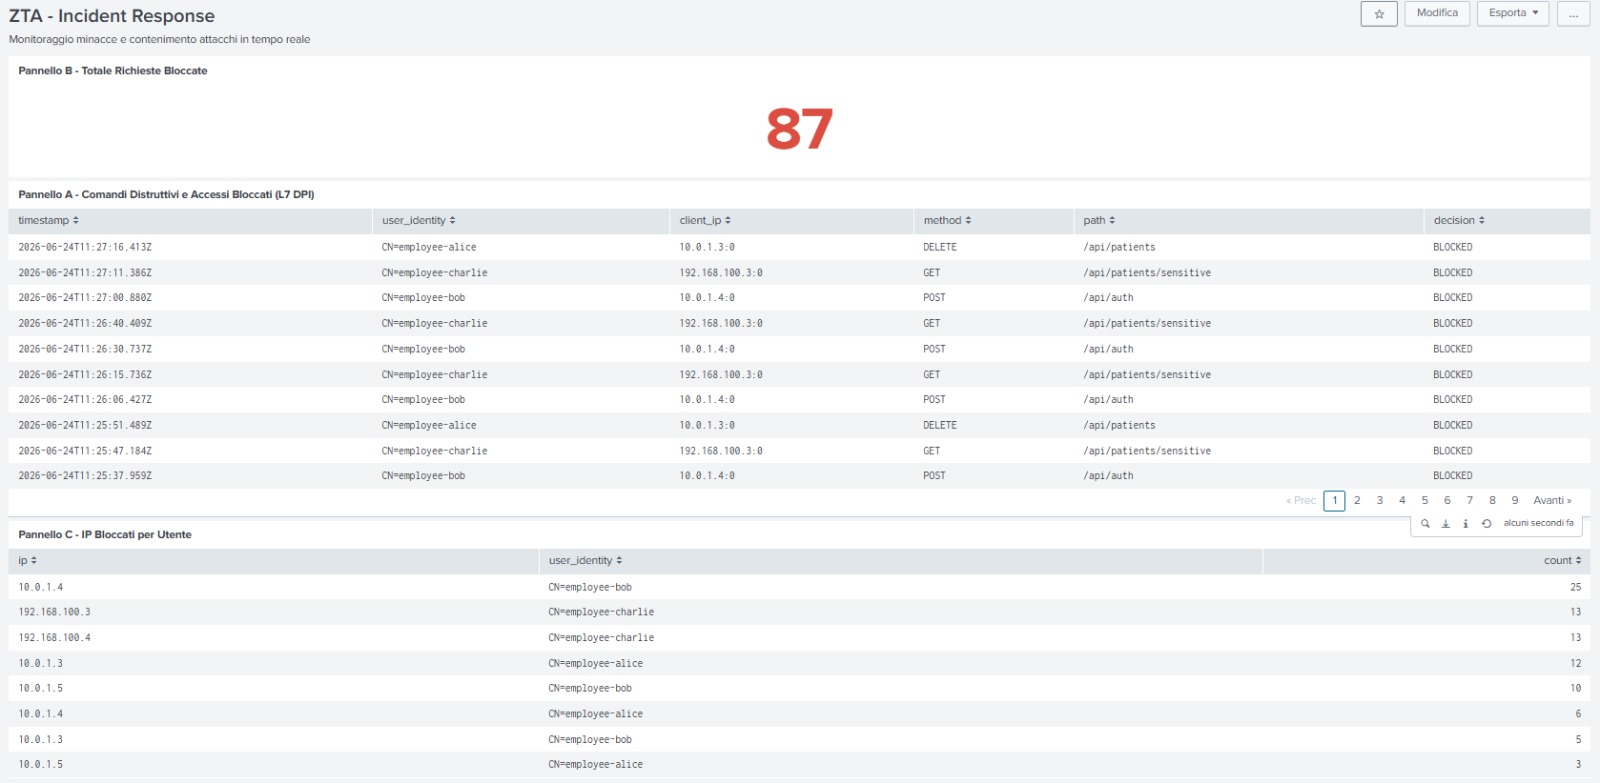
\includegraphics[width=1\textwidth]{capitolo4/img/dashboard2.jpeg}
    \caption{Dashboard ZTA - Incident Response: Monitoraggio minacce e blocchi attivi.}
    \label{fig:dashboard2}
\end{figure}

Infine, la dashboard ``ZTA - ML \& Continuous Trust Analytics'' (Figura \ref{fig:dashboard3}) espone le evidenze del modello di Machine Learning basato su Gradient Boosting. Il \textit{Pannello A} visualizza l'andamento del \textit{Risk Score} nel tempo per ciascun utente, permettendo di osservare la dinamica della fiducia: si noti come il punteggio di rischio (es. per l'utente \textit{charlie}) possa oscillare in risposta ad anomalie comportamentali. Il \textit{Pannello B} classifica gli utenti in base al rischio massimo raggiunto, fornendo un supporto decisionale critico per le procedure di isolamento automatizzato. Il \textit{Pannello C} integra infine i parametri di contesto --- frequenza delle sessioni, tentativi di login falliti e flag di attività in orario notturno --- che concorrono alla formulazione del calcolo dinamico del valore di rischio, chiudendo il ciclo di feedback tra il sistema di analisi e quello di autorizzazione.

\begin{figure}[H]
    \centering
    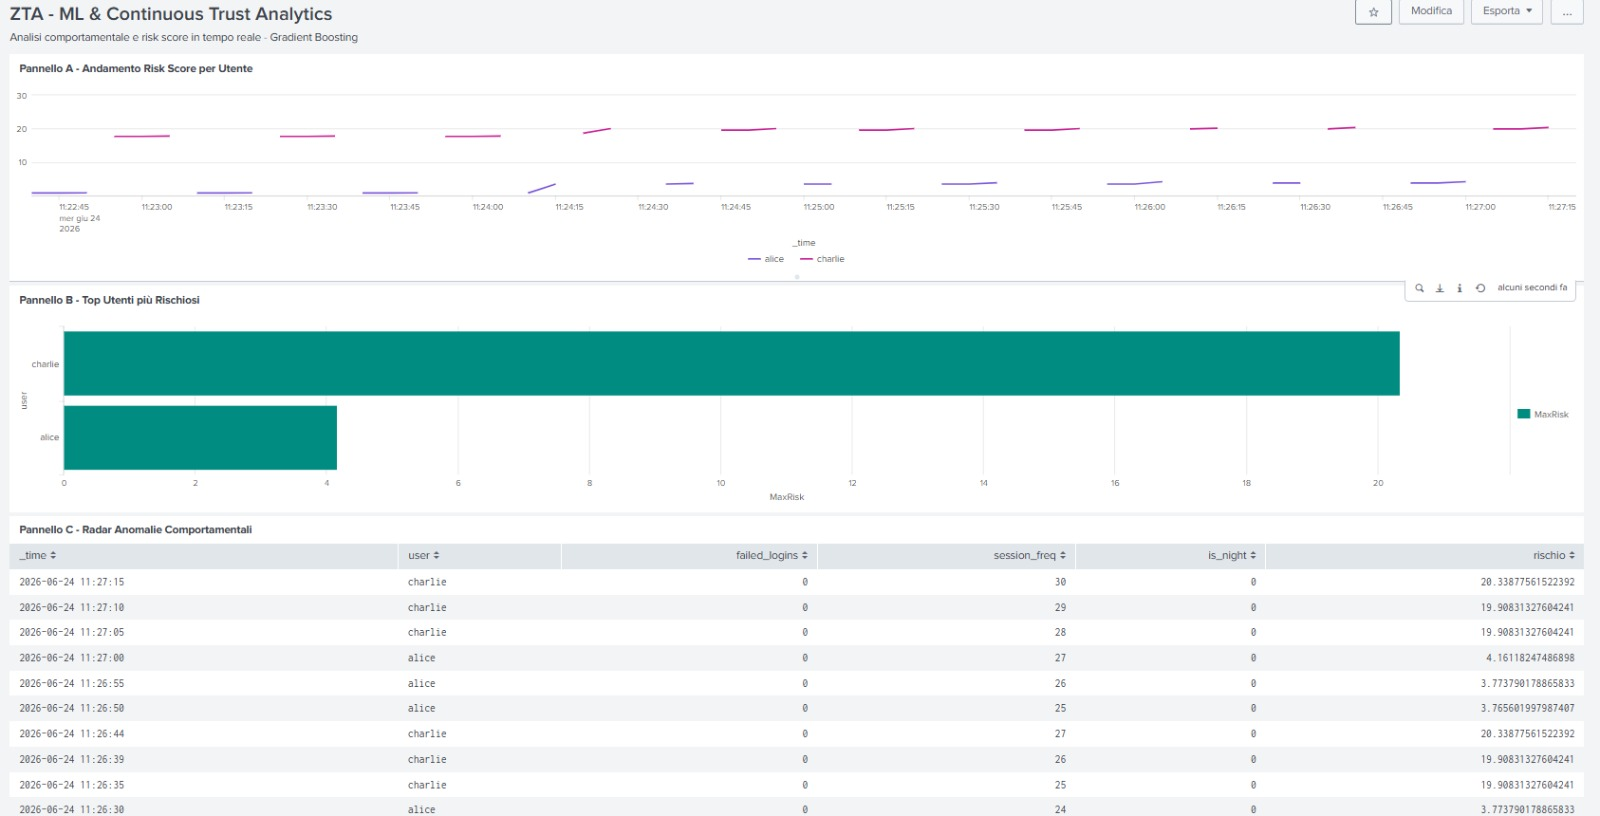
\includegraphics[width=1\textwidth]{capitolo4/img/dashboard3.jpeg}
    \caption{Dashboard ZTA - ML \& Continuous Trust Analytics: Analisi predittiva.}
    \label{fig:dashboard3}
\end{figure}